\documentclass{article}

\usepackage{graphicx}
\usepackage{hyperref}
\usepackage[a4paper, margin=1.25in]{geometry}
\usepackage{breakcites}
\usepackage{subcaption}
\usepackage{float}
\usepackage{textcomp}
\usepackage{amsmath}
\usepackage{textgreek}
\usepackage{authblk}
\usepackage{rotating}
\usepackage{booktabs}
\usepackage{longtable}
\usepackage{pdflscape}
\usepackage{lineno}
\usepackage[
  style=numeric,
  citestyle=numeric-comp,
  backend=biber,
  doi=true,
  natbib=true,
  sorting=none
]{biblatex}

\addbibresource{library.bib}

\begin{document}

\title{A Global Picture of Food Insecurity and Hunger}

\author[1,2,*]{Matthew Cooper}
\author[2,3]{Benjamin Müller}
\author[4]{Carlo Cafiero}
\author[2,5]{Juan Carlos Laso Bayas}
\author[2,6]{Homi Kharas}

\affil[1]{T.H. Chan School of Public Health, Harvard University}
\affil[2]{The World Data Lab, Vienna, Austria}
\affil[3]{Department of Economics, Vienna University of Economics and Business}
\affil[4]{The Food and Agricultural Organization of the United Nations}
\affil[5]{The International Institute for Applied Systems Analysis}
\affil[6]{The Brookings Institute}
\affil[*]{Corresponding Author: mcooper@hsph.harvard.edu}

\maketitle
\begin{abstract}
We modeled levels of of food security at a subnational level from 2010 to 2030 using microdata from 75 countries collected by the FAO and Gallup World Poll for the Voices of the Hungry project.  We find significant heterogeneity in levels of food security around the world, ranging from parts of the global north with less than 1\% of the population food insecure to parts of the global south where as much as 3 out of 4 people are severely food insecure.  Examining global temporal trends and accounting for the effects of the COVID-19 pandemic, we find that food insecurity has increased slightly over the past several years, but under middle-of-the-road assumptions for development and population change, food insecurity will decline throughout the 2020s.  This global decrease is largely driven by trends in South and East Asia, and some parts of the world, particularly sub-Saharan Africa, are projected to show increases in the prevalence of food insecurity throughout the next decade. Our model's forecast of decreasing food insecurity through the 2020s contrasts with predictions from the FAO that other metrics of hunger will increase.  This is the first global picture at a subnational level of the Food Insecurity Experience Scale, the food security metric most indicative of the lived experience of hunger.
\end{abstract}

\section{Main}
Food security is a critical component of human flourishing, which is why the second Sustainable Development Goal (SDG 2) is “Zero Hunger." One of the indicators to track progress on the first target of this goal, to ensure access by everyone to safe, nutritious and sufficient food (SDG2.1), is the prevalence of moderate to severe food insecurity in the population based on the Food Insecurity Experience Scale, or FIES. The FIES was developed by FAO in 2013 as a global extension of pioneering work done on Latin America to develop a metric of food insecurity based on the perspective of people who experience hunger and conditions that produce hunger. Other indicators of food insecurity, such as FAO's most commonly used estimate of undernourishment, are based on macro models of the mean and distribution of calories consumed per capita in a population. These do not capture the actual lived exposure of individuals to food shortages. 

Because the FIES is based on responses to polls, the data is limited to 75 countries where the polls have been conducted and microdata has been vetted and released by the FAO. The current practice is to assign the regional average prevalence rate for countries without survey data in order to compile regional and global aggregates. This is not very satisfactory. In addition, because the FIES is a relatively new metric, it does not have a sufficiently long time series to estimate trends with any degree of precision. To understand whether SDG 2 is being met, one needs to estimate food insecurity outcomes in 2030. 

The contribution of this paper is to fill these two gaps of coverage and forecasts by developing a model of FIES outcomes that is based on covariates that are available for places where actual polling data is not available, and that can be forecast to 2030 to get a sense of what food insecurity at that time might look like. We also take advantage of the within-country spatial distribution of FIES reports to push the analysis beyond country level to a sub-national level, that is administratively once removed from the national level (Admin-1). To our knowledge, this is the first effort to model the FIES outcomes at that scale.

Food security has traditionally been difficult to measure, and this has led to incomplete or inaccurate pictures of global hunger.  Metrics of macro-health, such as anthropometry and mortality rates are correlated broadly with food insecurity and have been used for many years to monitor human well-being \citep{Puffer1973, Habicht1974}.  However, these metrics are confounded with other determinants of health such as infectious disease and are not meaningful at the scale of individuals or households \citep{Perumal2018}.  Other proxies for food security, such as food availability estimated from crop yields \citep{Maxwell1992}, are also inadequate because they only make rough estimates of how accessible food is to the general population, and food insecurity can certainly occur in the absence of food availability decline \citep{Sen1983}.  Moreover, these metrics are very sensitive to incorrect estimates of crop yields and food reserves at a national scale.  Thus, global estimates of hunger and food insecurity based on these metrics carry forward similar flaws.

As researchers began to focus on food insecurity at the individual and household level, household microdata collecting information on household finances and consumption became a common proxy for food security \citep{Haddad1994}.  However, these efforts were criticized for being onerous, insufficiently comparable, as well as for ignoring subjective and experiential aspects of food security \citep{Maxwell1996}.  This led to the emergence of several indicators designed to be rapidly deployable, and based on the lived experience of food security \citep{Jones2013}.  These metrics include the Household Food Security Survey Module (HFSSM) \citep{kennedy2005keynote}, originally developed for use in the US; the Latin American and Caribbean Food Security Scale (ELCSA); and the Household Food Insecurity and Access Scale (HFIAS) \citep{Coates2007}.

Drawing on the insights derived in designing and implementing these novel food security metrics, the FIES was developed by the Food and Agricultural Organization (FAO) of the UN \cite{Ballard2013} and is now recognized as a rapidly deployable and cross-culturally valid tool for understanding individual and household-level food insecurity \citep{wambogo2018validity, smith2017world}.  The FIES is based on a survey of eight behaviors indicative of food insecurity and hunger over the previous year, such as skipping meals or worrying about having enough to eat.  Using a Rash model \citep{Cafiero2018}, each individual in the survey is given a severity score that maximizes the likelihood of observing he responses given to the 8 questions asked in the survey.  Once individuals are ranked in this fashion, thresholds for moderate and severe food insecurity are set that describe people's experiences, and the prevalences can be computed. A moderately food insecure adult is likely to have compromised on food quality and variety, as a result of lack of income, has been unsure about their ability to obtain food and has skipped meals or run out of food occasionally. A severely food insecure adult is likely to have run out of food and has gone an entire day without eating at times during the year.  Because the model estimates the population over a threshold on a univariate food insecurity scale, the percentage of people over the threshold for moderate food insecurity includes people that are also over the threshold for severe food insecurity.

Since 2014, in partnership with Gallup World Poll, the FAO administered the FIES in surveys around the world. The FAO uses this data to estimate the prevalence of food insecurity, and reports national-level estimates of the percentage of the population over the thresholds for moderate and severe food insecurity.  Drawing on individual-level data from these microdatasets in 75 countries, we used machine learning to estimate levels of food insecurity around the world at the subnational level.  The model is then used to infer levels of food insecurity around the world at the subnational level and to forecast food insecurity to the year 2030.

\section{Results}
\subsection{Food Insecurity over Time}
Globally, in the year 2020, we estimate that 829 million people are above the threshold for severe food insecurity, and an additional 1.5 billion people are above the threshold for moderate food insecurity (See Fig. \ref{fig:timeseries}). These numbers are higher than the estimates in the 2019 FAO State of Food Insecurity report, which estimated about 700 million severely food insecure people and an additional 1.31 billion people experiencing at least moderate food insecurity in 2018. 

While the total number of people experiencing moderate and severe food insecurity held roughly constant for the 2010s and even increased in latter part of that decade, our model predict that it will decline throughout the 2020s. However, this overall decline will not be uniform across the world. Our model expects that, in most of sub-Saharan Africa, moderate food insecurity will increase throughout the 2020s and severe food insecurity will plateau, although some countries, such as Kenya, Ethiopia, and Ghana, will see improvements. Food insecurity will fall in most other world regions, particularly South Asia and East Asia \& the Pacific.

\begin{figure}[H]
  \centering
  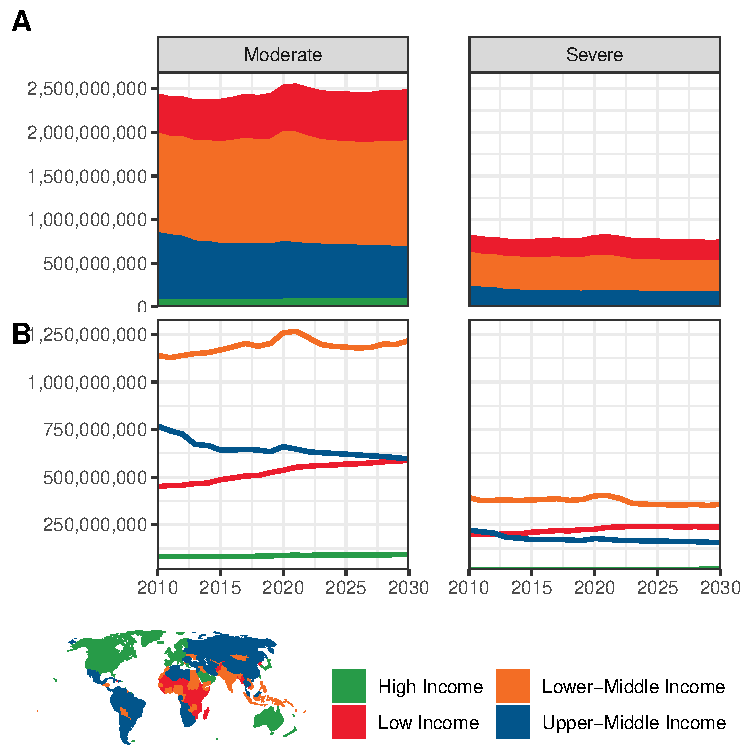
\includegraphics[width=\linewidth]{img/TimeSeries.pdf}
  \caption{Number of people over the thresholds for moderate and severe food insecurity, by UN SDG regions over time, with a 3-year smoothing.  Panel (A) shows the number of food insecure people with region totals stacked, to show global trends and totals over time.  Panel (B) shows regional totals compared against each other over time.}
  \label{fig:timeseries}
\end{figure}

Examining the rate of food insecurity in a population, rather than the total number of food insecure people (See Fig. \ref{fig:rates}, our model finds the most progress has been made in East \& Southeast Asia, while Central \& Southern Asia is expected to see improvements in food insecurity throughout the 2020s.  Other poor and middle income areas, including much of Africa, the Middle East and Latin America, have made only slight progress and will continue to make slight progress between 2010 and 2030.  In high-income countries in Europe and North America, rates of people in at least moderate food insecurity move little, and rates of severe food insecurity are expected to increase slightly.  Overall, the world has made has made steady but slow progress on reducing the rate of food insecurity.

\begin{figure}[H]
  \centering
  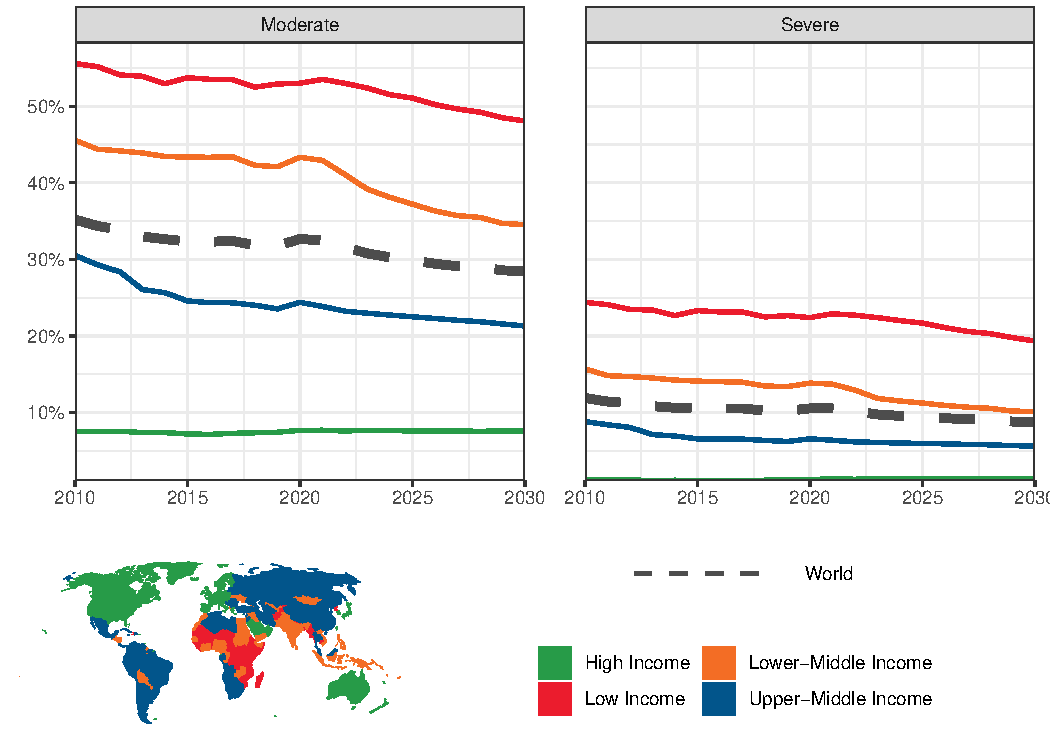
\includegraphics[width=\linewidth]{img/Rates.pdf}
  \caption{Percentage of the population over the threshold for moderate and severe food insecurity, by UN SDG regions over time, with a 3-year smoothing.}
  \label{fig:rates}
\end{figure}


\subsection{Food Insecurity over Space}
We found substantial heterogeneity in the global distribution of severe food insecurity (See Fig. \ref{fig:map}).  For the year 2020, mainland sub-Saharan Africa is the continent with with the highest rates of severe food insecurity, with at least 15\% of people over the threshold for severe food insecurity in at last one subnational area in every country except Gabon and Equatorial Guinea.  Outside of Africa, serious pockets of severe food insecurity also occur in Venezuela, Syria, Papua New Guinea, Yemen, and Afghanistan.  In many large middle-income countries, severe food insecurity is also quite prevalent, with rates between 10-15\% in areas like northern Brazil, many central Asian and middle-eastern countries, and India and Indonesia.

The experience of at least moderate food insecurity is quite common in many parts of the world.  In 2020, much of Africa, south and southeast Asia, and parts of Latin America had over 50\% of the population living with moderate food insecurity.  Even in countries widely considered to be developed, such as Australia, the United States, and parts of eastern and southern Europe, over 10\% of the population is above the threshold for moderate food insecurity.  

\begin{landscape}
\begin{figure}[h]
  \centering
  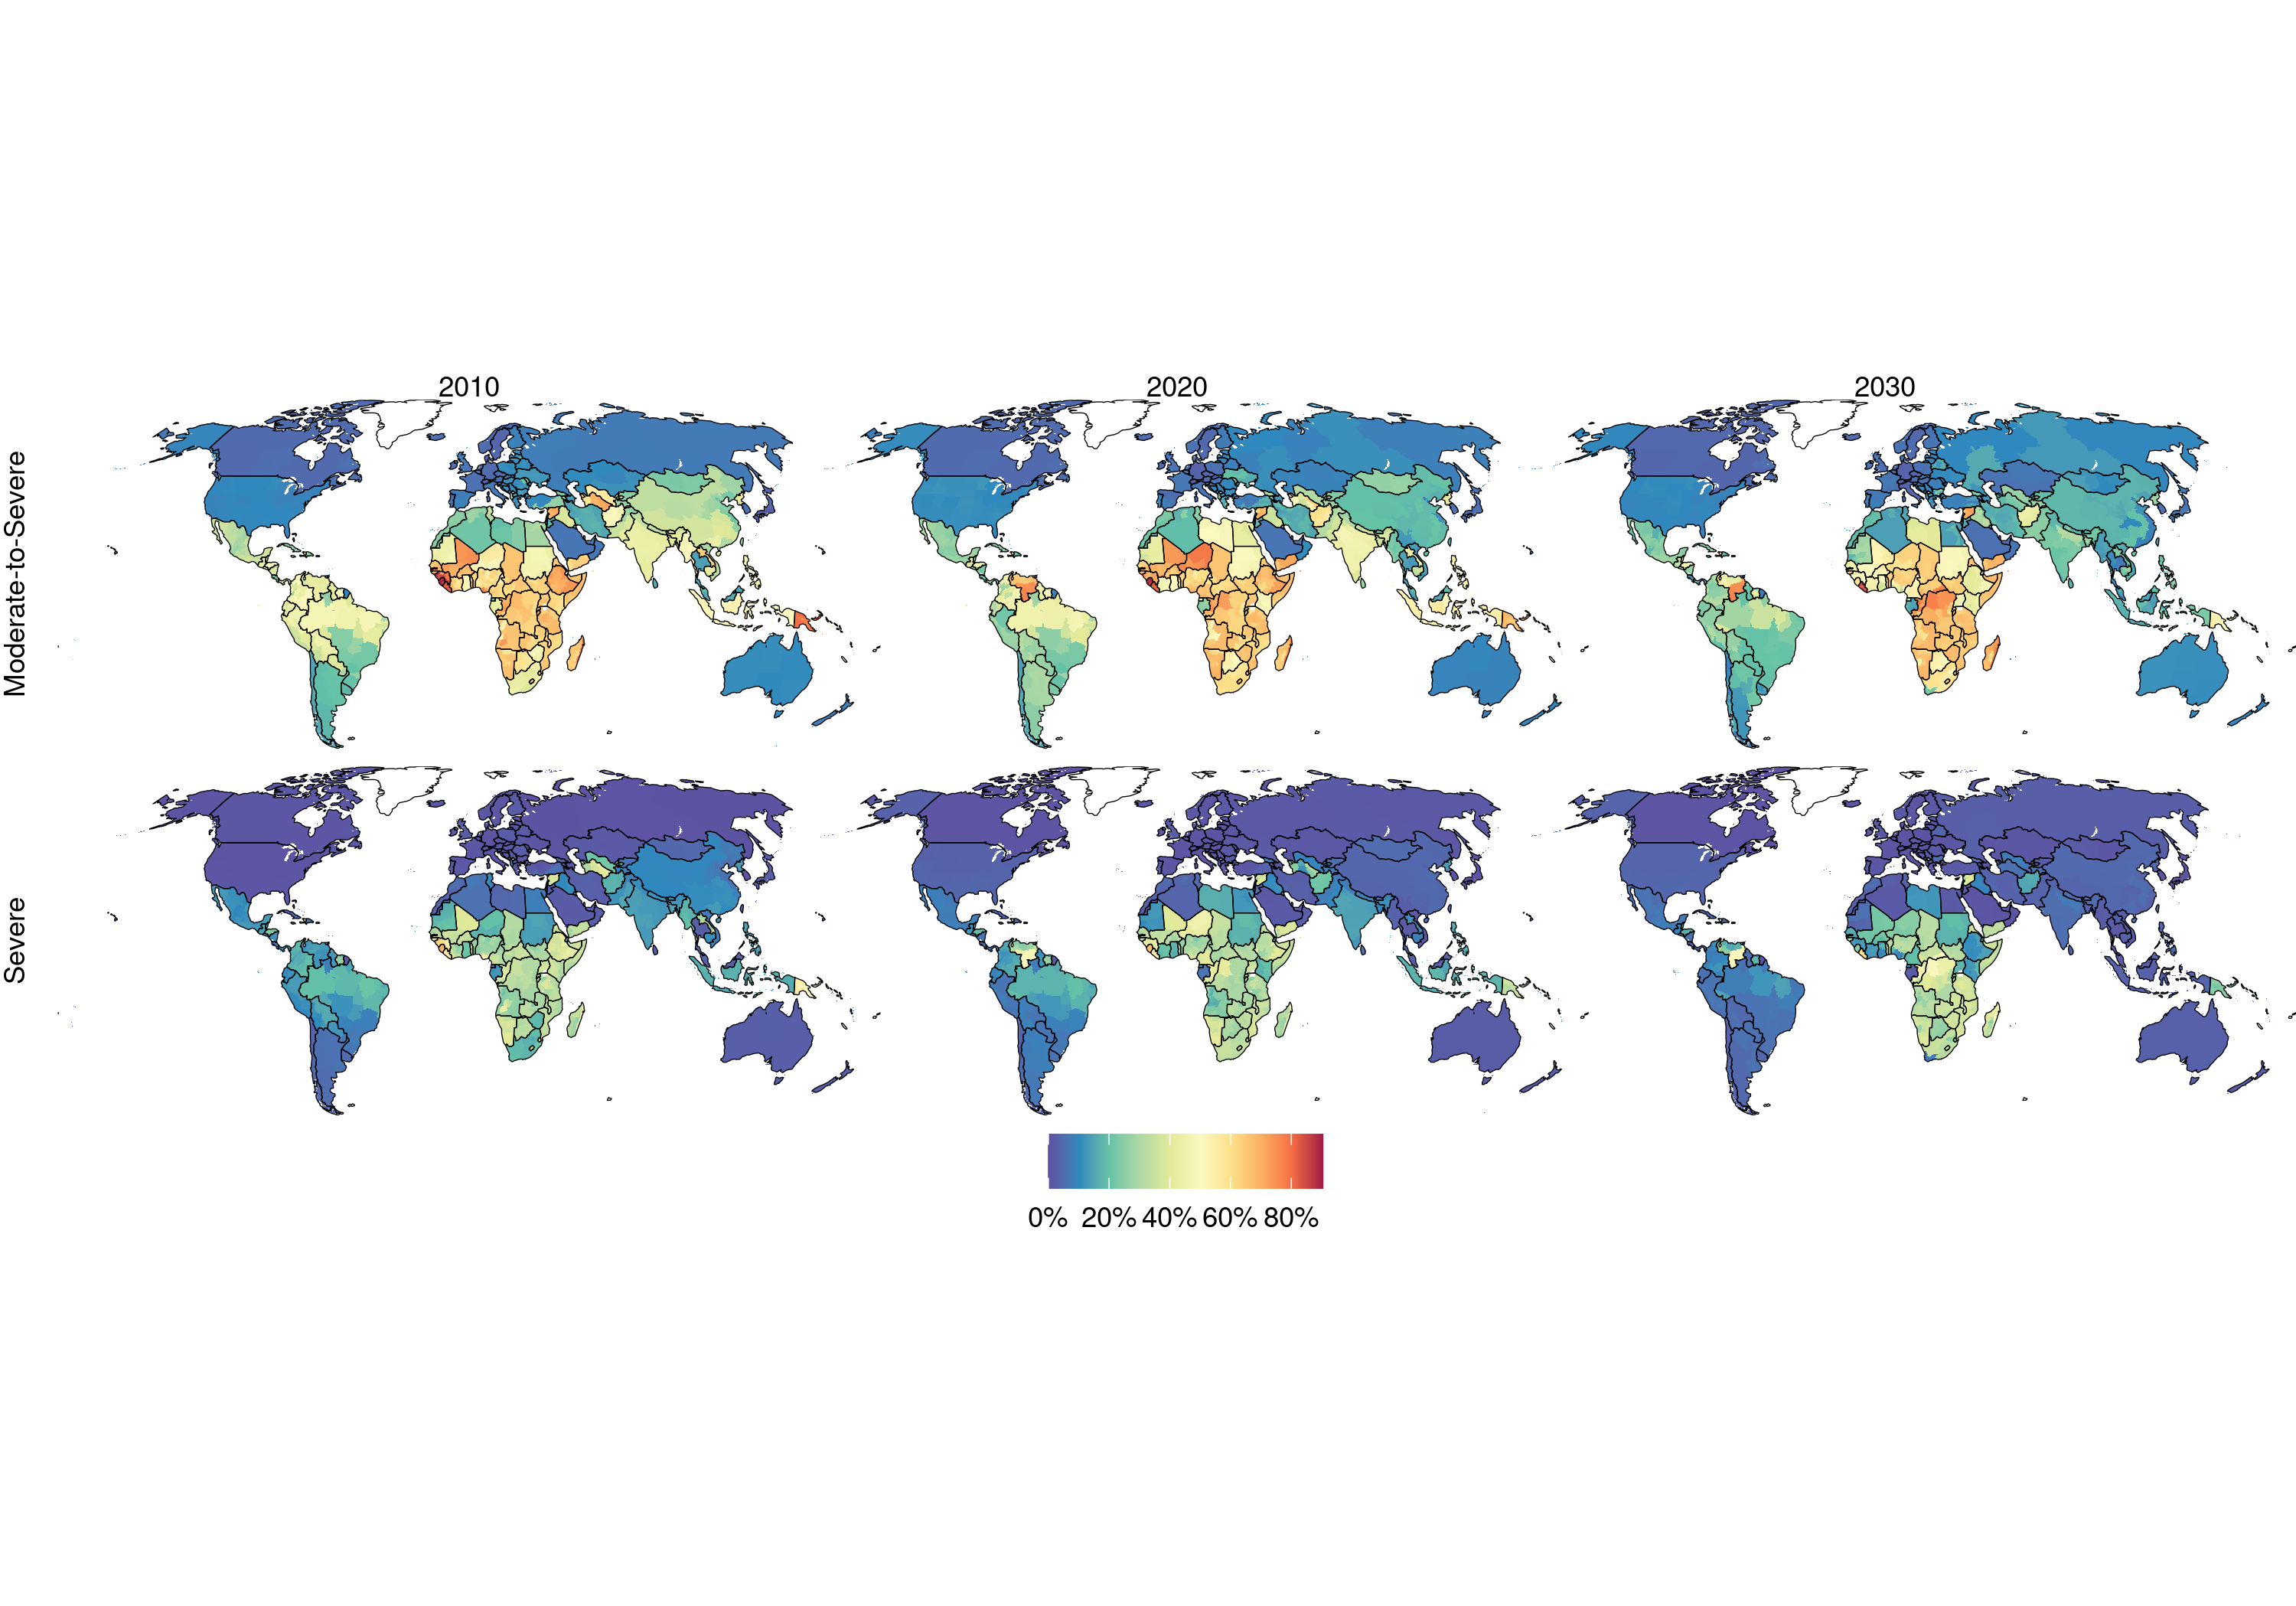
\includegraphics{img/FullMap.png}
  \caption{Modeled spatial distribution of moderate and severe food insecurity for the years 2010, 2020, and 2030.}
  \label{fig:map}
\end{figure}
\end{landscape}

\subsection{Important Predictors of Food Insecurity}
Overall, our model was able to predict food insecurity with high accuracy in the countries that had training data ($R^2 = 0.9981$ and $R^2 = 0.9976$ for moderate and severe food insecurity, respectively).  Examining how permuting a variable affects the predictive accuracy of the model can give an idea of how important that variable is for predicting food insecurity.  

For both moderate and severe food insecurity, the most important variable for predicting food security levels was the Poverty Headcount Index, followed by the rate of stunting.  For predicting the rate of people with at least moderate food insecurity, GDP per capita was quite important.  However, for the rate of severe food insecurity, the country's Gini coefficient was more important compared to moderate food insecurity.

\begin{figure}[h]
  \centering
  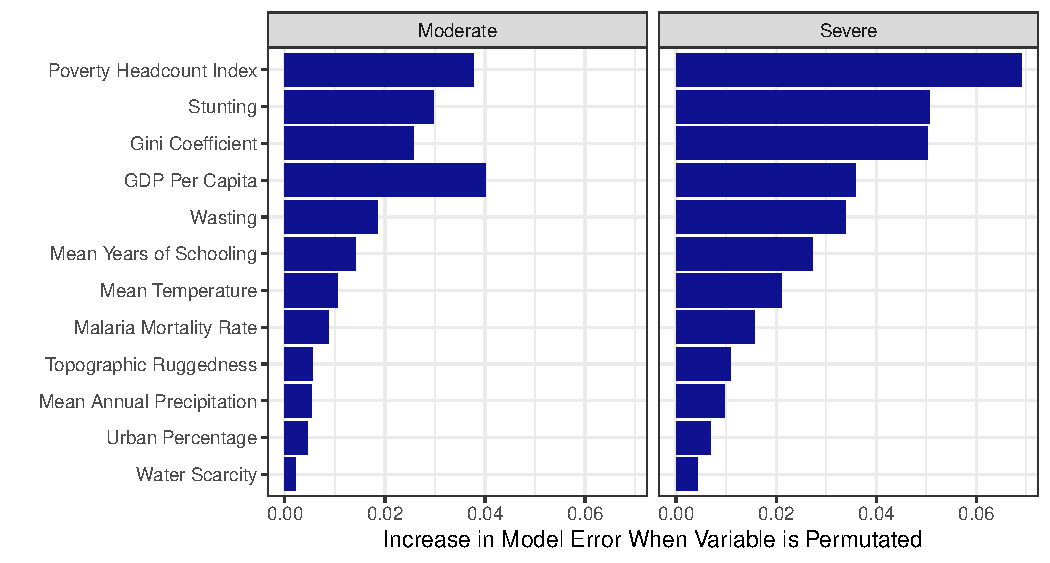
\includegraphics[width=\linewidth]{img/VIMP.pdf}
  \caption{Importance of each variable in predicting the percent of a population over thresholds for moderate and severe food insecurity.  This is determined by the increase in the error when the variable is permuted before fitting the model.}
  \label{fig:map}
\end{figure}


The results of this analysis can be further explored in more detail on the \href{https://worldhunger.io}{World Hunger Clock}, including statistics for each subnational administrative area.

\section{Discussion}
This paper presents the first global estimates of the experience of food insecurity at a subnational level, with forecasts out to the year 2030.  We found that, while food insecurity has been increasing and has likely worsened in 2020 with economic downturn associated with the novel coronavirus, our models predict that number of people who experience food insecurity globally will decrease throughout the 2020s, largely because of progress in south and east Asia.  Nevertheless, many regions, most notably sub-Saharan Africa, are expected to see overall increases in the number of food insecure people. 

Our variable importance metrics show that economic conditions are the largest driver of global variation in rates of food insecurity.  For both moderate and severe food insecurity, the poverty headcount index, the Gini coefficient, and GDP per capita were major predictors of the rate of food insecurity.  The rate of stunting, an indicator of both sanitary conditions and chronic, long-term hunger was also an important predictor of food insecurity.  However, other indicators of sanitary conditions, such as the rates of wasting and malaria mortality were less important predictors of food insecurity.  Geographic and climate factors, such as urban percentage, topographic ruggedness and mean annual temperature and precipitation were not important predictors of food insecurity at a global scale.  Finally, while economic conditions are widely associated with food insecurity at a global scale, the fact that Europe and North America is predicted to see little improvement in food insecurity outcomes between 2010 and 2030, in spite of economic growth and continued reductions in poverty, suggests that there is an upper limit to the extent to which increasing economic development can improve food security outcomes.

These results contrast with the FAO's predictions of increased rates of undernourishment, the other indicator for the SDG 2 target of ending hunger \citep[Part 1, Page 11]{sofi2020}.  This is likely due in part to our differing modeling approaches. While the SOFI report extrapolated recent trends in undernourishment and stunting, we modeled food insecurity based on interactions between projections in factors like GDP per capita, population, and the prevalence of stunting. Additionally, our diverging predictions for different SDG 2 indicators are not necessarily mutually exclusive: it is theoretically possible for undernourishment to increase while food insecurity, as measured by the FIES, decreases.  The discrepancies between our projections illustrate both how hunger is a complex phenomenon that is resistant to simple quantification, as well as the challenges in forecasting the future, where different modeling approaches will yield different predictions.

When making predictions in countries where we did not have primary data, we are assuming that the relationship between variables like poverty, stunting, inequality, and hunger are the same in all locations.  We tested the accuracy of these cases by using ten-fold cross validation at the country level, and we found reasonable accuracy ($R^2 = 0.778$, MAE = 0.073 for moderate and $R^2 = 0.696$, MAE = 0.044 for severe food insecurity).  This suggestions that our model explains between 70-78\% of the variation in food security outcomes and is on average, within 4-7\% in its estimates of rates of food insecurity, when applied to countries outside of the training set. 

Additionally, when making predictions into the future, we are assuming that long-term patterns of demographic change, urbanization, and development will maintain their long-held trajectories for the next decade.  At a global scale, this is almost certainly the case: it is highly unlikely that rates of fertility or economic growth with shift suddenly and globally.  Nevertheless, at more local scales, sudden crises can lead to severe and unforeseeable increases in food insecurity, as crises in the previous decade in Yemen, Syria and Venezuela have shown.  Thus, while our model's predictions at a global scale are very likely to bear out, there will probably be individual countries and areas where our forecasts end up being off.

While we found that food insecurity will decrease overall by 2030, our model, which relies on middle-of-the-road assumptions, only expects the number of people experiencing moderate food insecurity to fall by 12\% and the number of people experiencing severe food insecurity to fall by 20\%.  This still leaves billions of people eating less than they should and nearly half a billion people going entire days without eating a decade from now, a number that falls far short of the SDG 2 goal of ending hunger.  Moreover, decreases in food insecurity as measured by the FIES do not necessarily mean there will be improvements in other significant challenges such as poor dietary quality, micronutrient deficiencies, or obesity.  Thus, while expected trends in correlates of food security give cause for optimism, there is still significant work to be done in pursuit of SDG 2.

\section{Methods}

%do we need to add a section where we state which fies data we use? like countries and years?

\subsection{Disaggregation}
The data on the FIES collected by Gallup records many individual-level attributes from the respondents, including age, gender, wealth quintile, and whether they live in an urban or rural area.  Using national data on these variables, a standard weighting scheme is created for each individual, based on the ratio of population probabilities to sample probabilities of an individual with those characteristics being selected \citep{bethlehem2009applied}.  We used a similar methodology, except we calculated post-stratification weights at a subnational level.  We used year-specific subnational estimates of population percentages by gender, age, urbanization, and, where available, wealth, and created a separate set of weights for each subnational area across all individuals.  For age and gender, we used gridded data from WorldPop \citep{Tatem2017}, for urbanization, we used spatially explicit estimates published by Jones and O'Neill \citep{Jones2016}, and for wealth we used data on household wealth quintiles from Demographic and Health Surveys \citep{dhsall}, where available.  This methodology rests on the mild assumption that subnational differences in rates of food insecurity are more due to factors related to demographics, urbanization, and wealth than to other unobservable factors.

\subsection{Covariates}
We model subnational rates of severe and moderate-to-severe food insecurity as a function of several covariates related to human development, food security, health, infrastructure, income levels and distribution, and the environment (See Table \ref{tab:covars}).  We aimed for covariates that had subnational spatial resolution and peer-reviewed projections available through the year 2030.   For projections based on the Shared Socioeconomic Pathways (SSP) framework \citep{oneill2014new}, we used the middle-of-the-road pathway, SSP2, and for climatological variables, we use forecasts based on Representative Concentration Pathway (RCP) 6.0 \citep{van2011representative}.  

Many of the variables required harmonizing subnational historic data with projections at the national level.  This included mean years of schooling, GDP per capita, as well as for projections of population. We used observed trajectories in the historical distribution of variables among subnational areas within a country to estimate the future distribution of GDP, population, and schooling among subnational areas and disaggregate national-level future projections.

In cases of health variables that have shown long-term trends and represented a rate of occurrence in a population, including stunting, wasting, and malaria mortality rate, we estimate the Annualized Rate of Change (AROC) for each subnational area to model these variables for 2030. The involves taking the rate of change between each pair of years in the dataset, and then taking the mean rate of change over the period for which data is available, giving greater weight to more recent years, and applying that mean rate of change to estimate future levels.  This method has been used to estimate rates of stunting and wasting in 2025 \citep{Local2020}; we simply use the same method to make forecasts to the year 2030.

For the climate variables temperature and precipitation, we combined historical observations with an ensemble of four bias-corrected simulations of the future climate from the Inter-Sectoral Impact Model Intercomparison Project (ISIMIP) \citep{warszawski2014inter}.

Finally, we adjusted several variables to account for the effects of COVID-19, including GDP per capita using June 2020 estimates from the World Bank \citep{prospects2020}, stunting and wasting using August 2020 estimates published in \textit{The Lancet} \citep{headey2020impacts}, as well as the poverty headcount index \cite{Cuaresma2018}.  For a detailed overview of the steps involved in processing and preparing each covariate, see the Appendix.

\begin{table}[H]
  \centering
	\begin{tabular}{lll}
		\toprule
    Name & Source & Scale \\
		\midrule
    Urban Percentage & \citep{Jones2016} & Subnational \\
    Stunting & \citep{Local2020} & Subnational \\
    Wasting & \citep{Local2020} & Subnational \\
    Mean Years of Schooling & \citep{Smits2019, KC2017} & Subnational\\
    GDP Per Capita & \citep{Smits2019, Dellink2017} & Subnational \\
    Gini Coefficient & \citep{Rao2019a} & National\\
    Poverty Headcount Index & \citep{Cuaresma2018} & National \\
    Water Scarcity & \citep{greve2018global} & Subnational \\
    Mean Annual Precipitation &  \cite{abatzoglou2018terraclimate, warszawski2014inter} & Subnational \\
    Topographic Ruggedness &  \cite{USGS1996, Riley1999} & Subnational \\
    Mean Temperature &  \cite{abatzoglou2018terraclimate, warszawski2014inter} & Subnational \\
    Malaria (\textit{P. falciparum}) Mortality Rate &  \cite{Weiss2019} & Subnational \\
		\bottomrule
	\end{tabular}
	\caption{Covariates Included in Present-Day Analysis}
	\label{tab:covars}
\end{table}


\subsection{Modeling}
We fit two models for all subnational areas globally from 2010 to 2030: one for the percent of the population over the threshold for moderate food insecurity, and one for the percent of the population over the threshold for severe food insecurity.  We used random forest regressions, as this approach performs well in the presence of non-linearities and important interactions among predictor variables \citep{hastie2009elements}.  A random forest regression involves generating a large number of decision trees, each under slightly different conditions and using different sub-samples of the data, and then aggregating the predictions of the decision trees.

Because the outcome variables in our models, the rate of moderate or severe food insecurity, are a bounded outcome, we first used a logistic transformation to extend the range from $[0,1]$ to $(-\infty, \infty)$.  Then, after estimating the model, we used the inverse logit to convert the unbounded model predictions to a rate between 0 and 1.

To get the best possible model performance, it is necessary to tune the hyperparamters, which control the process in which the random forest algorithm is run.  Key hyperparameters include the number of decision trees to generate, the number of variables randomly selected as candidates for splitting a node, and the average number of observations in a leaf node.  We calculated the Out-Of-Bag (OOB) error for different combinations of hyperparameters for the moderate and severe models. By choosing the combinations of hyperparameters with the smallest OOB error we found the optimal combination for both models. We found that 5000 trees are more than sufficient for the error rates to converge.

After fitting the models, we examined the importance of the individual covariates in explaining rates of moderate and severe food insecurity. We used a common method of permuting each individual variable and re-running the regressions, and then determining the difference in Mean Average Error (MAE) between the regression \citep{ishwaran2007variable}.  Similarly to model predictions, we transformed the error term with the inverse logit so that the errors would be on the scale of the outcome variable and therefore more interpretable.

\subsection{Model Validation}
We observed a MAE of 0.0029 for our model of severe food insecurity ($R^2$ of 0.9978) and an MAE 0.0054 for our model of moderate food insecurity ($R^2$ of 0.9981).  This means that, on average, our model predictions were only of by 0.29\% and 0.54\%, respectively, for the subnational areas in countries where we had microdata. 

To further validate the models, we ran a ten-fold cross validation at the country level.  We randomly divided the countries into ten parts, and re-fit the model 10 times, with each part left out one.  Then, we predicted the values for the ten percent that was left out using the model fit with 90\% of the countries.  We randomly left out data at the country level because within each country we had values from different subnational areas and different years, and these values are likely to be very similar to each other.  Because we are extending our models predictions to countries that were not found at all in our training data, a better test of our model is to assess its predictive accuracy on countries that were entirely absent from the training data.  By this validation metric, we found that our model performed reasonably well, with an $R^2$ of 0.778 and an MAE of 0.073 for moderate food insecurity and an $R^2$ of 0.696 and a MAE of 0.044 for severe food insecurity.

For a detailed description, implementation and validation of the random forest models see the Supplemental Info.

\section{Conclusion}

\printbibliography

\section*{Supplemental Info}
\setcounter{table}{0}
\setcounter{figure}{0}
\setcounter{section}{0}
\renewcommand{\thetable}{S\arabic{table}}
\renewcommand{\thefigure}{S\arabic{figure}}
\renewcommand{\thesection}{S\arabic{section}}

\section{Overview of the FIES}
We used raw microdata released by the FAO from 75 countries that vary by world region and income level (See Fig. \ref{fig:fies_countries}.

\begin{figure}[H]
  \centering
  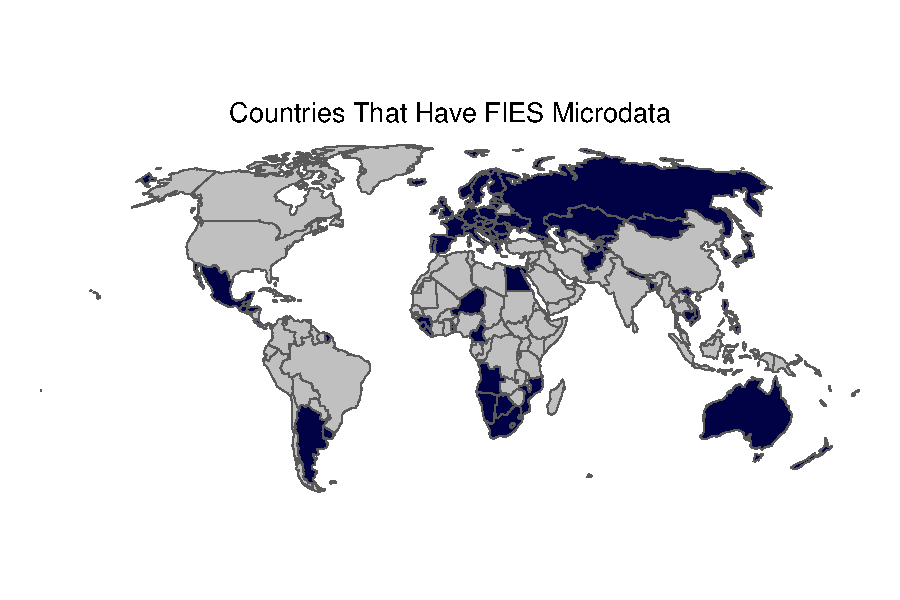
\includegraphics[width=\linewidth]{img/FIES_Countries.pdf}
  \caption{Countries that had microdata on the FIES and were used in our model, shown in blue.}
  \label{fig:fies_countries}
\end{figure}

This microdata comes with the probability that an individual is over the threshold for moderate and severe food insecurity already calculated by the FAO, based on their responses to the 8 FIES questions (See List \ref{itm:fies}).  Thus, we did not perform those calculations ourselves.  Nevertheless, we give here an overview of the procedure.  For more detail see Cafiero (2018) in \textit{Measurement} \citep{Cafiero2018}.

The FIES is calculated using a Rash model, which was developed by the psychometrics literature.  The Rash model assumes that each individual and their responses to the FIES questions can be placed on a one-dimensional scale of food insecurity, and that the log odds of a respondent \textit{r} answering yes to one of the FIES questions \textit{i} is a linear function of the difference between the severity of the food insecurity experienced by \textit{r} and the severity of item {i}.

The severity of each item and each respondents level of food insecurity can be estimated with Maximum Likelihood.  After fitting the model to each country, the FAO found that the assumptions of the Rash model held up well, as evidenced by model fit diagnostics.

After separately estimating the Rash model for each country, the FAO then developed a global reference scale for the severity of each of the 8 questions, by iteratively harmonizing the severity values in each country.  Then, these global reference points were calibrated against other surveys that had asked questions similar to the FIES, such as the HFSSM and the ELCSA.

Based on the global reference scale, two thresholds are set based on questions 1 and 8: whether the responded was worried they would not have enough food to eat because of a lack of money or other resources, and whether there was a time when they went without eating for a whole day because of a lack of money or other resources.



%%% Discuss reference scale and calibration
%%% Map of countries with Training Data
\begin{enumerate}
	\item During the last 12 MONTHS, was there a time when you were worried you would not have enough food to eat because of a lack of money or other resources?
	\item Still thinking about the last 12 MONTHS, was there a time when you were unable to eat healthy and nutritious food because of a lack of money or other resources?
	\item Was there a time when you ate only a few kinds of foods because of a lack of money or other resources?
	\item Was there a time when you had to skip a meal because there was not enough money or other resources to get food?
	\item Still thinking about the last 12 MONTHS, was there a time when you ate less than you thought you should because of a lack of money or other resources?
	\item Was there a time when your household ran out of food because of a lack of money or other resources?
	\item Was there a time when you were hungry but did not eat because there was not enough money or other resources for food?
	\item During the last 12 MONTHS, was there a time when you went without eating for a whole day because of a lack of money or other resources?
  \label{itm:fies}
\end{enumerate}

\section{Predicting Covariates Into the Future}
\subsection{Annualized Rate of Change}
For many of our covariates, to extrapolate recent trends to the future, it is necessary to draw on annualized rates of change, which are then used to anticipate the rate of future change.  This method can be used for any variable that is a fraction or a rate.  We use this method to estimate future rates of stunting, wasting, and malaria mortality, as well as to model future subnational shares of GDP and population.  Thus, we give an overview of the methodology here.

First, for each subnational area, $a$, the rate of change (ROC) is calculated between each pair of adjacent years, $y$, based on a value, $p$, such that $0 < p < 1$, available for each year.

\begin{equation}
  \text{ROC}_{a,y} = \text{logit} \left( \frac{p_{a,y}}{p_{a,y-1}} \right)
  \label{eqn:a}
\end{equation}

Then, each ROC is weighted to give more weight to recent years, such that weight $W$ at year $y$ is.  For a dataset with observations for 2010 to 2017, that would be:

\begin{equation}
  W_y = \frac{y - 2010}{\sum_{y=2010}^{2017} y - 2010}
  \label{eqn:b}
\end{equation}

Then, the annualized rate of change (AROC) is calculated as:

\begin{equation}
  \text{AROC}_{a} = \text{logit} \left( \sum_{y=2010}^{2017} W_y \times \text{AROC}_{a, y} \right)
  \label{eqn:c}
\end{equation}

Finally, the projections, Proj, for each year from 2018 to 2030 are given as:

\begin{equation}
  \text{Proj}_{a,y} = \text{logit}^{-1} ( \text{logit} ( p_{a,2017} ) + AROC_{a} \times ( y - 2017 ) )
  \label{eqn:d}
\end{equation}

For cases where we are modeling shares of a whole, for example when modeling subnational shares of population or GDP, we then re-scale the shares to ensure they total to 1.

\subsection{Population}
Although population is not a covariate in our random forest model, it is an important precursor to other covariates, such as GDP per capita, and future estimates of population are also necessary to convert modeled future rates of food insecurity into total headcounts of food insecurity.  Thus, in addition to our other covariates, we also modeled population into the future.

We do this by combining historic subnational data from the Subnational Development Database \citep{Smits2019} with national level population estimates for the 21st century \citep{KC2017}.  To account for within-country trends and changes in population distribution, we use the AROC method outlined in equations \ref{eqn:a} - \ref{eqn:d} to project each subnational areas share of national population totals. We then disaggregate the national totals given by KC et al. to estimate future subnational populations.

\begin{figure}[H]
  \centering
  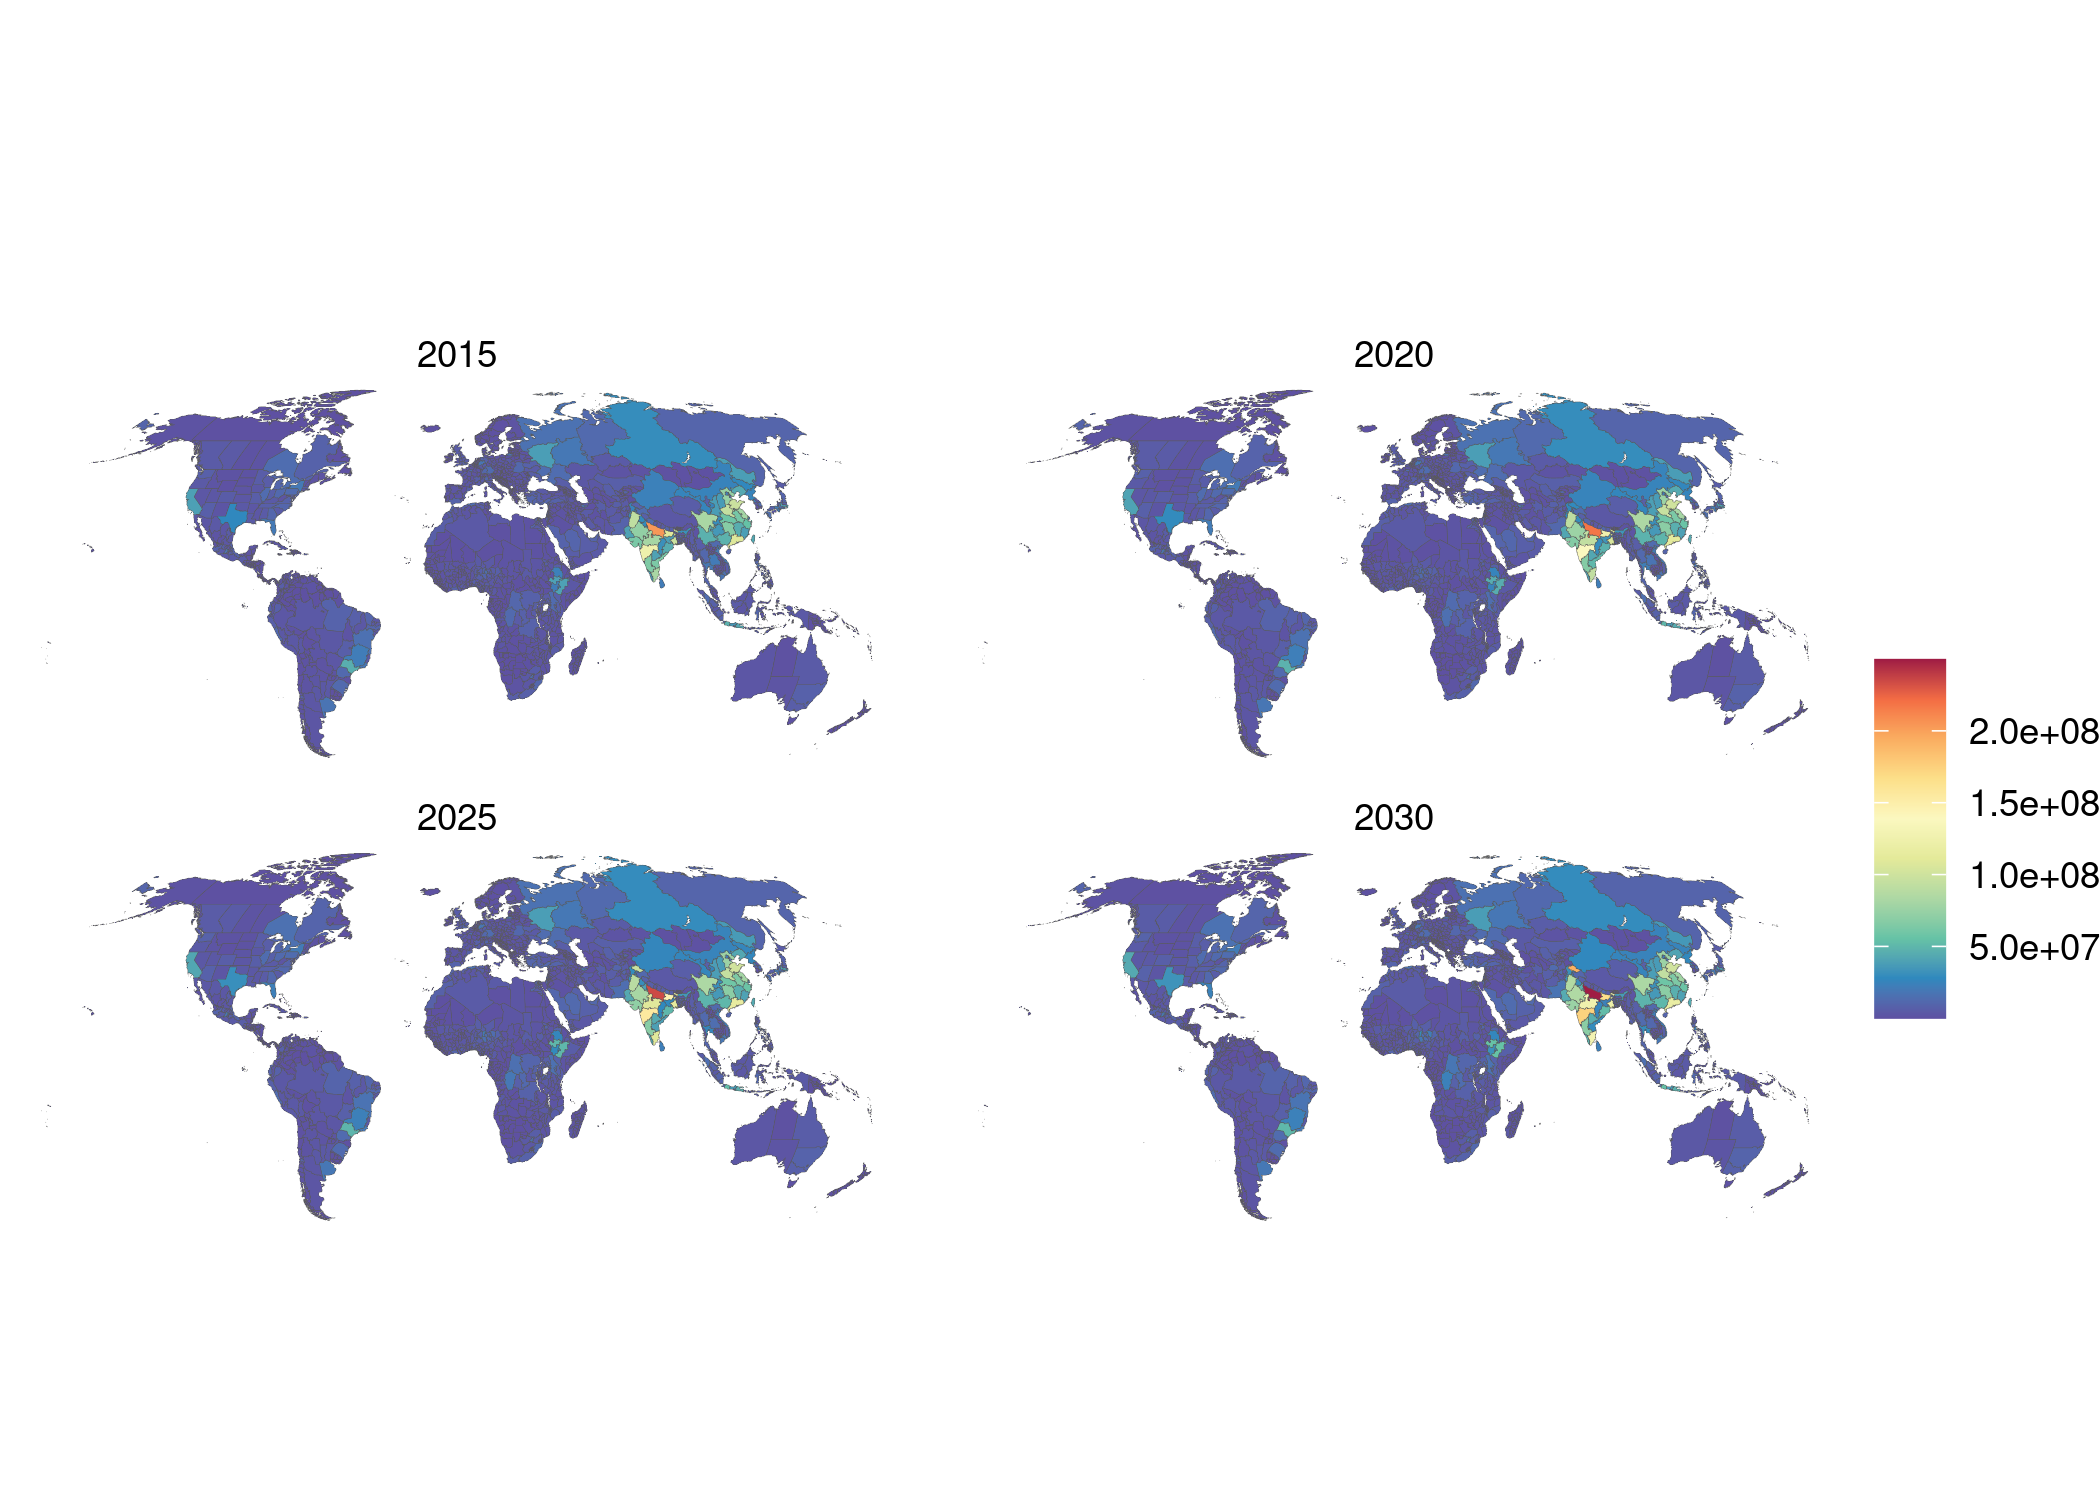
\includegraphics[width=\linewidth]{img/covars/population.png}
  \caption{Population}
\end{figure}

\subsection{Urban Percentage}

We drew our historic and future estimates of urbanization entirely from Jones and O'Neill, published in \textit{Environmental Research Letters} \citep{Jones2016}, who modeled spatially explicit scenarios of urbanization consistent with the Shared Socioeconomic Pathways.  As with our other covariates, we used estimates for SSP2, the middle-of-the-road scenario.  Because definitions of ``urban" and ``rural" vary significantly across datasets, using one dataset that is entirely consistent within itself was an important consideration.

\begin{figure}[H]
  \centering
  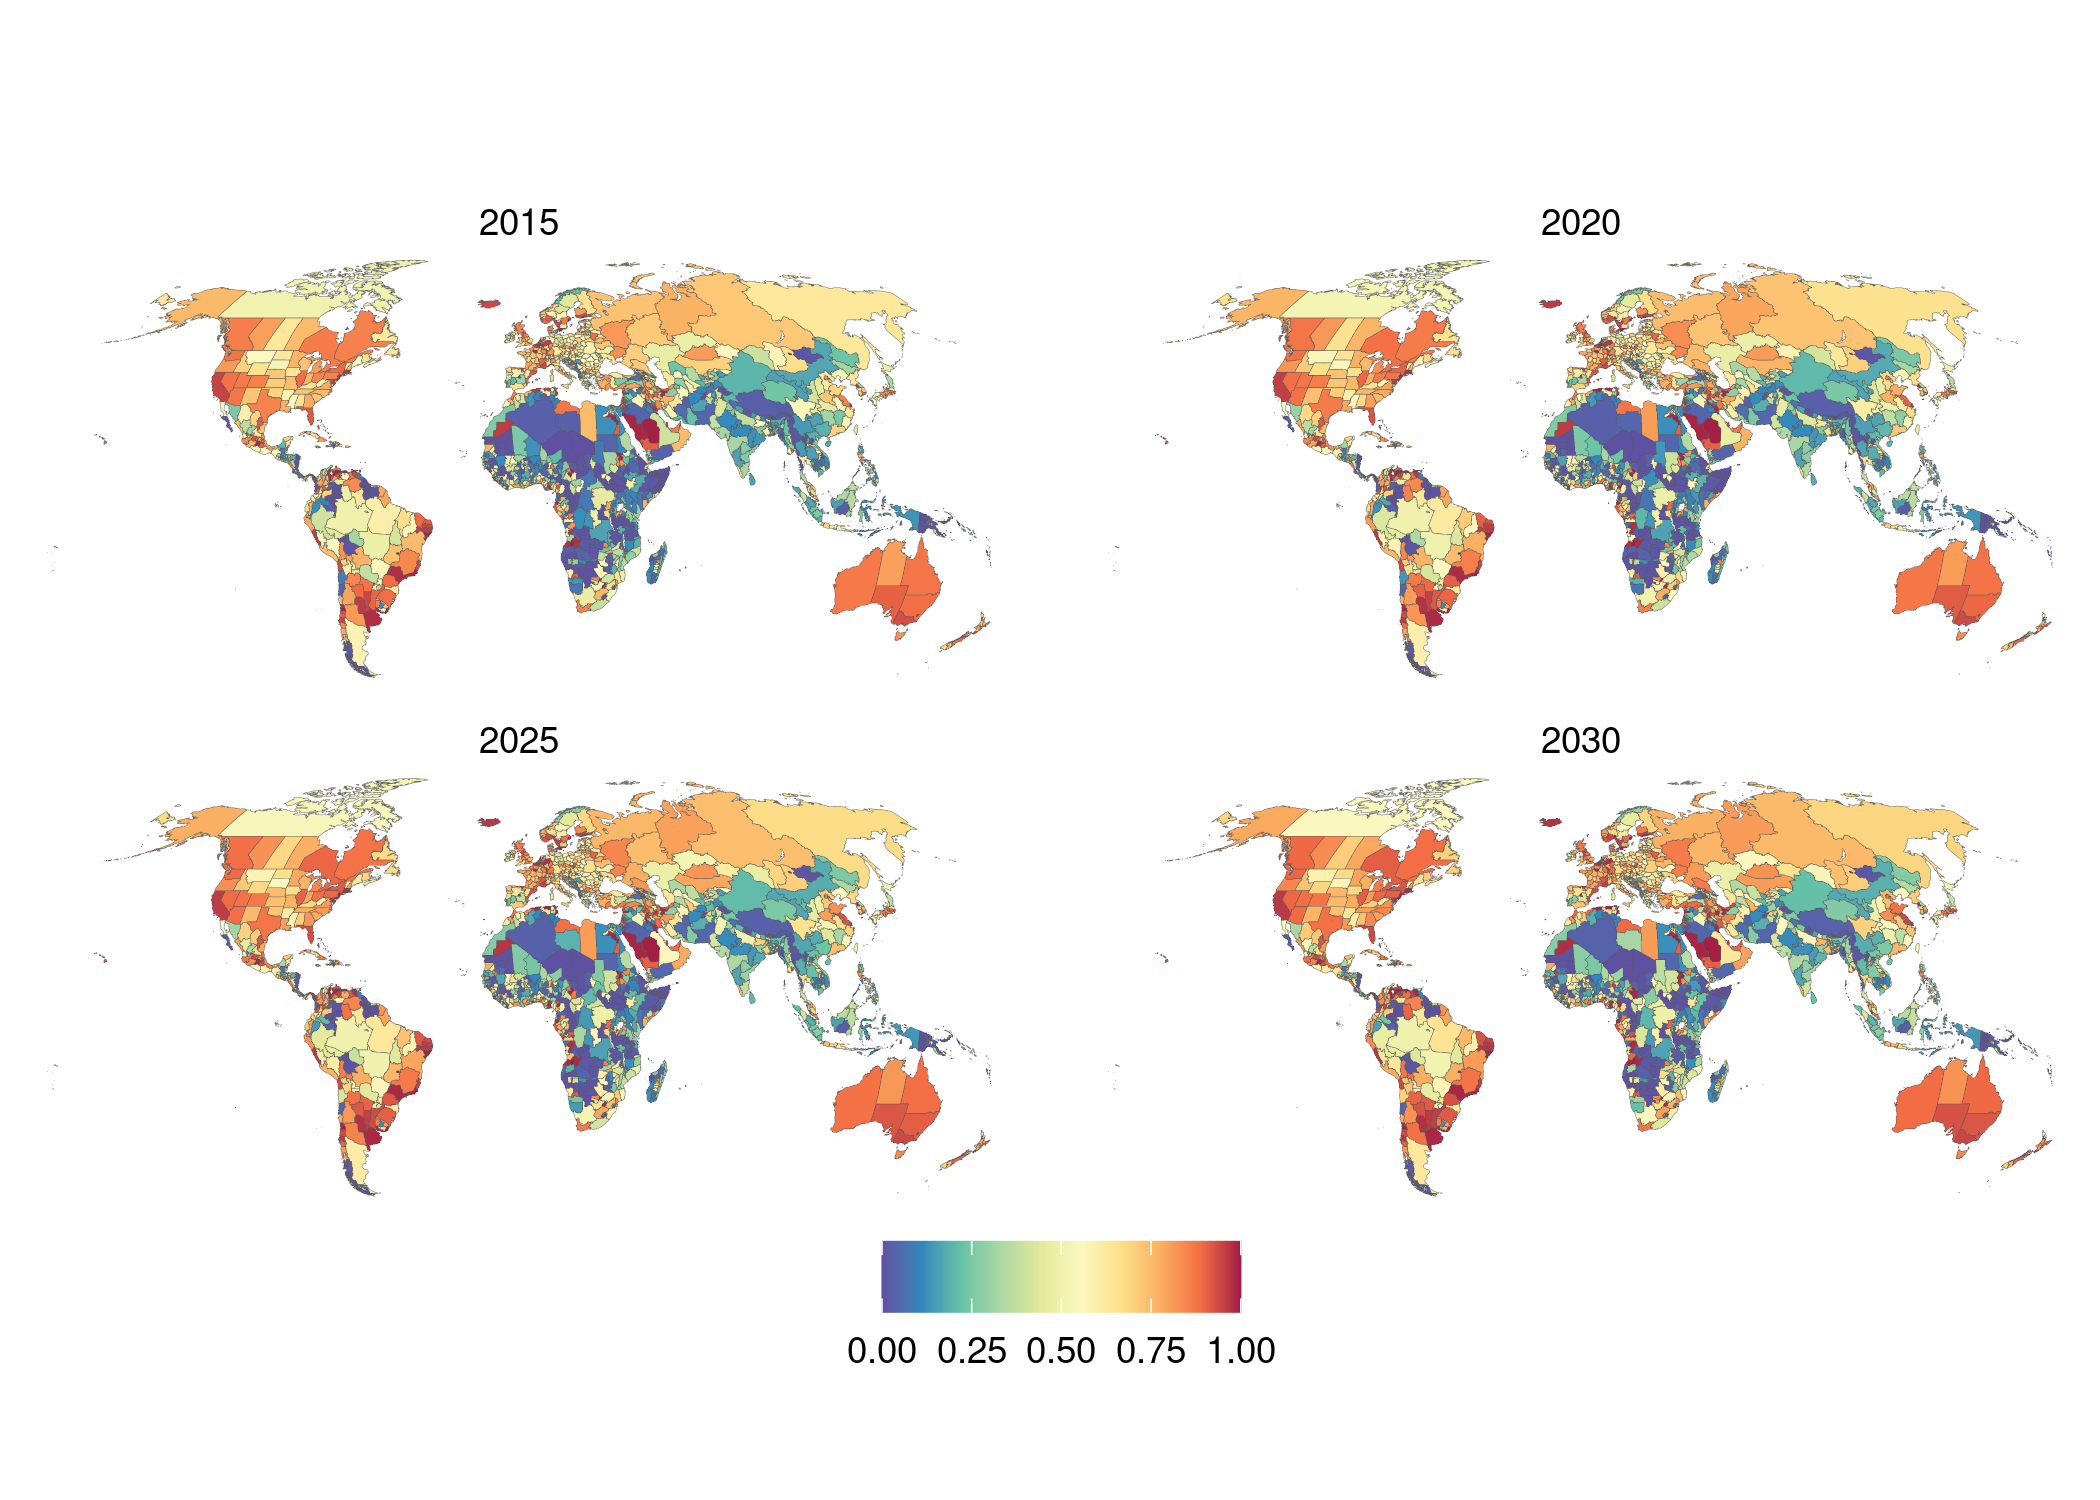
\includegraphics[width=\linewidth]{img/covars/urban_perc.png}
  \caption{Percentage of people living in urban areas.}
\end{figure}

\subsection{Wasting}
To estimate the prevalence of wasting for each administrative area in our dataset, we used data from the Local Burden of Disease project published in \textit{Nature} \citep{Local2020}.  For the years 2010 to 2017, we simply took the mean rate of wasting in each administrative area from the dataset.  Higher-income countries that were not included in the dataset were modeled as having a rate of 0 wasting.  We then modeled wasting for the years 2018-2030 using the AROC method, which the Local Burden of Disease group similarly used to estimate wasting for the year 2025 \citep{Local2020}.

To account for the effects of the novel coronavirus on global rates of wasting, we assumed that long-term trends and rates of wasting would hold steady, but that they increase globally by 14.3\% in 2020, based on estimates published in \textit{The Lancet} \citep{headey2020impacts}.  We model this impact as uniform across all countries where wasting occurs.  Then we model the rate of wasting in each administrative area in 2021 as being the mean of the rate in 2020 that accounts for the shock and the previously modeled rate for 2022.

\begin{figure}[H]
  \centering
  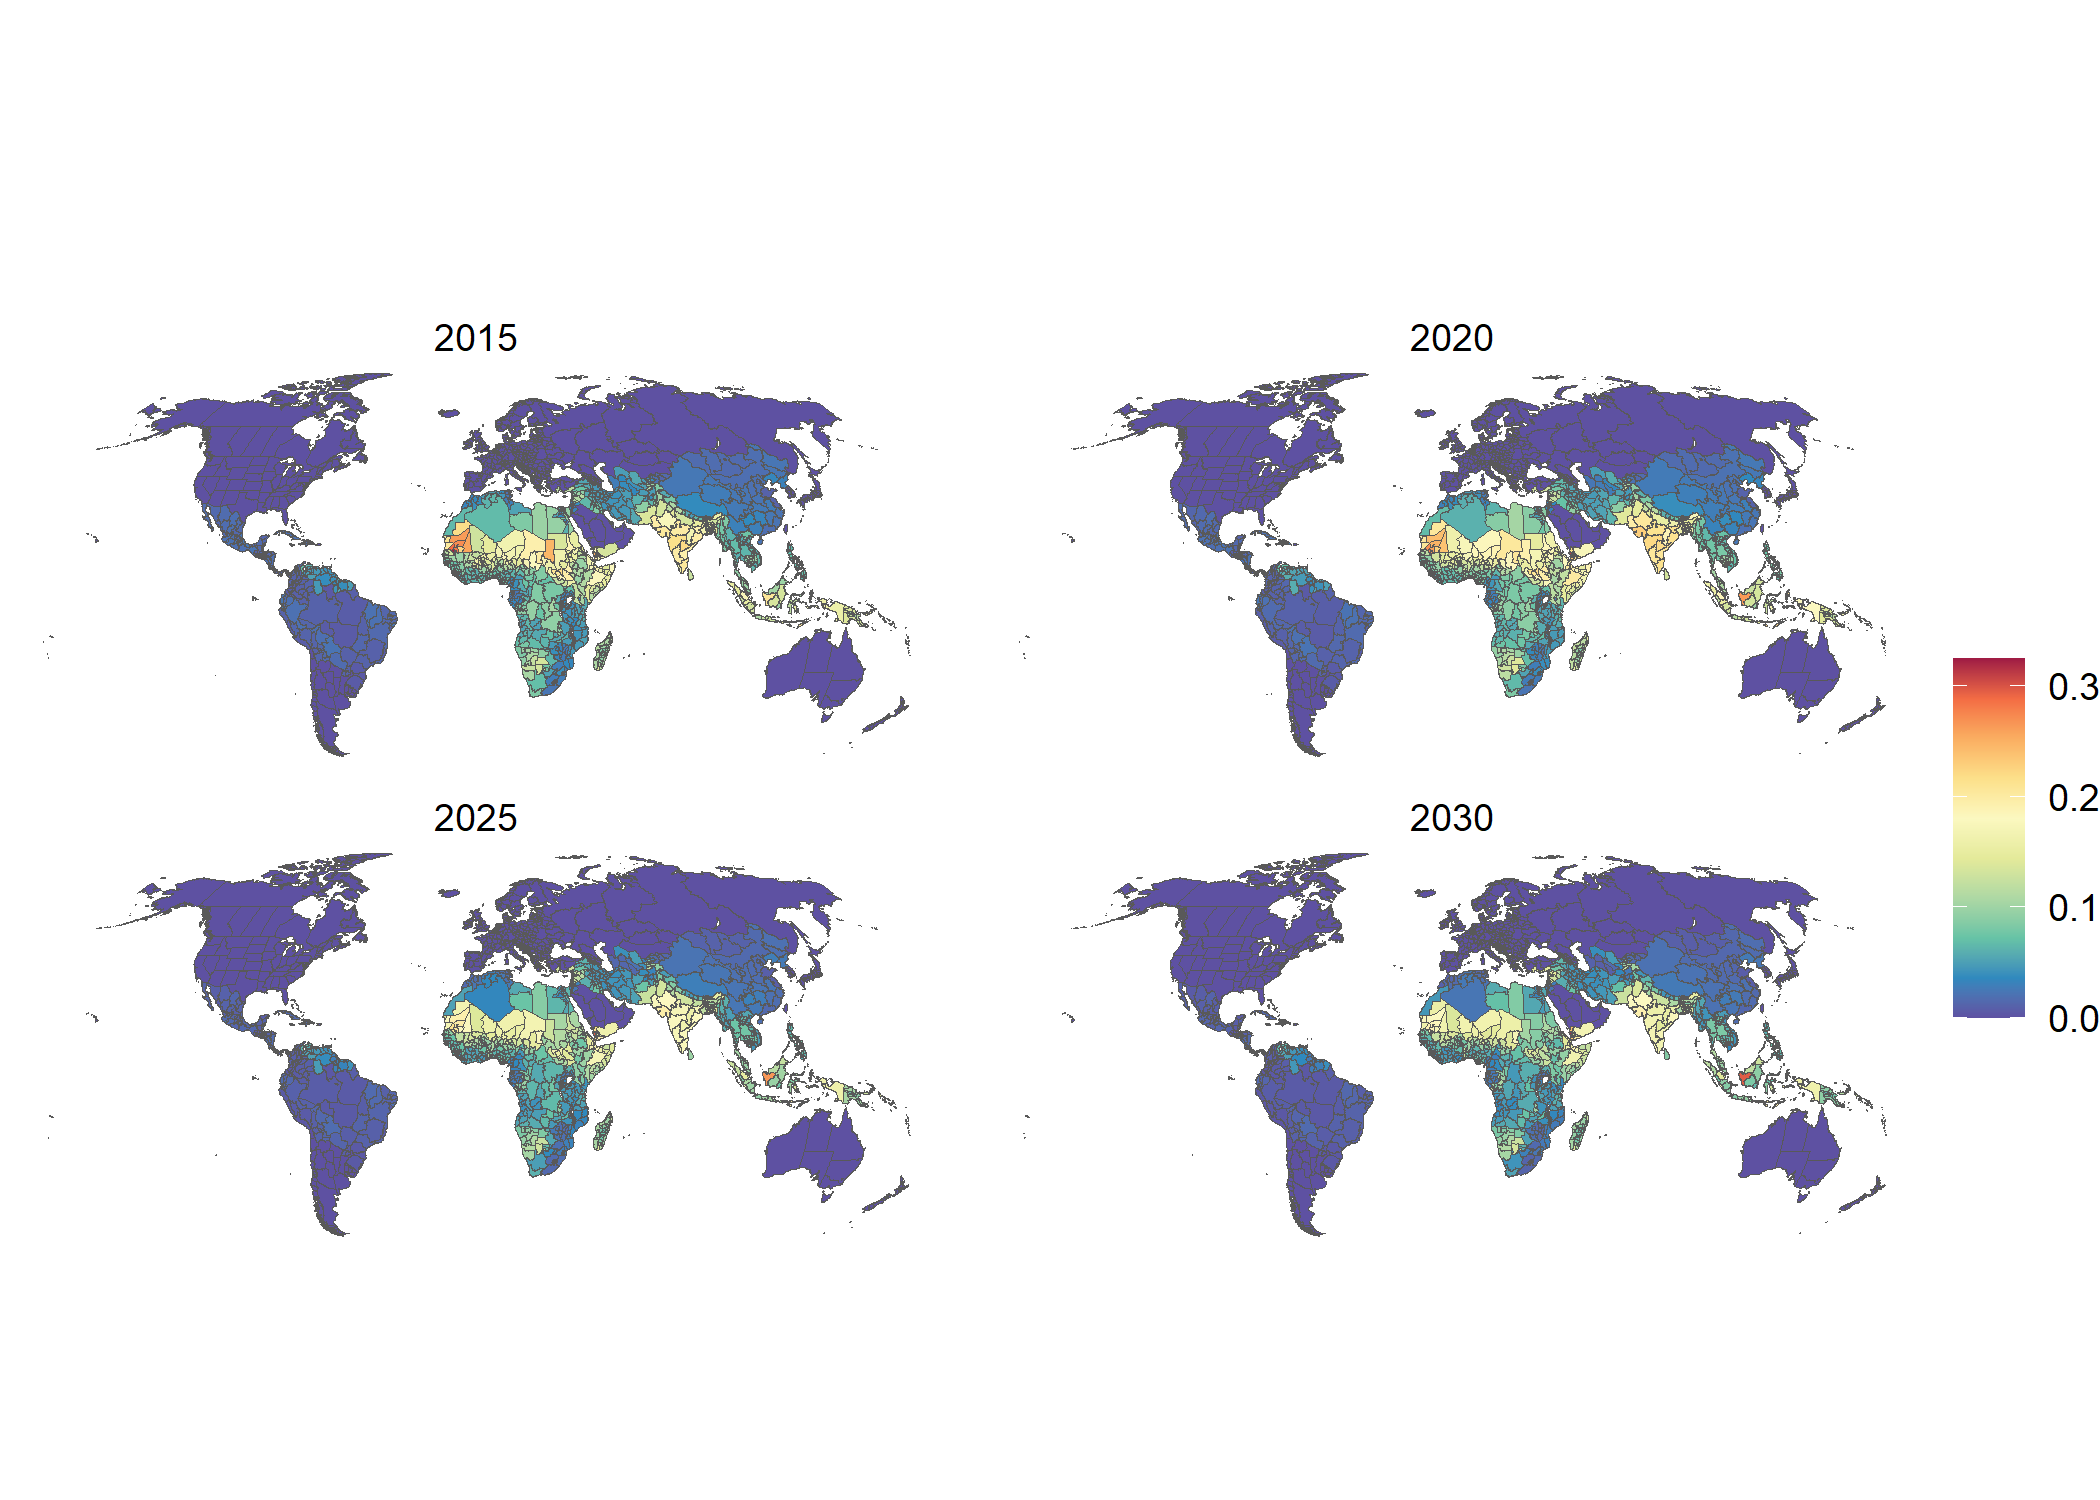
\includegraphics[width=\linewidth]{img/covars/wasting.png}
  \caption{Prevalence of wasting.}
\end{figure}

\subsection{Stunting}

We model stunting using the same methodology we use to summarize and model wasting, because the Local Burden of Disease dataset that we draw on for wasting also includes stunting.  We also included the 14.3\% increase in prevalence for the year 2020 that was estimated for wasting \citep{headey2020impacts}, even though stunting is a long-term consequence of malnutrition and will likely not be as readily observable in a population as wasting would be.  However, we use stunting in our model not as a cause of food insecurity, but rather as a proxy for chronic conditions of hunger, which are exacerbated by the coronavirus pandemic.  Thus, estimating an impact of the coronavirus shock on stunting is appropriate for our model.

\begin{figure}[H]
  \centering
  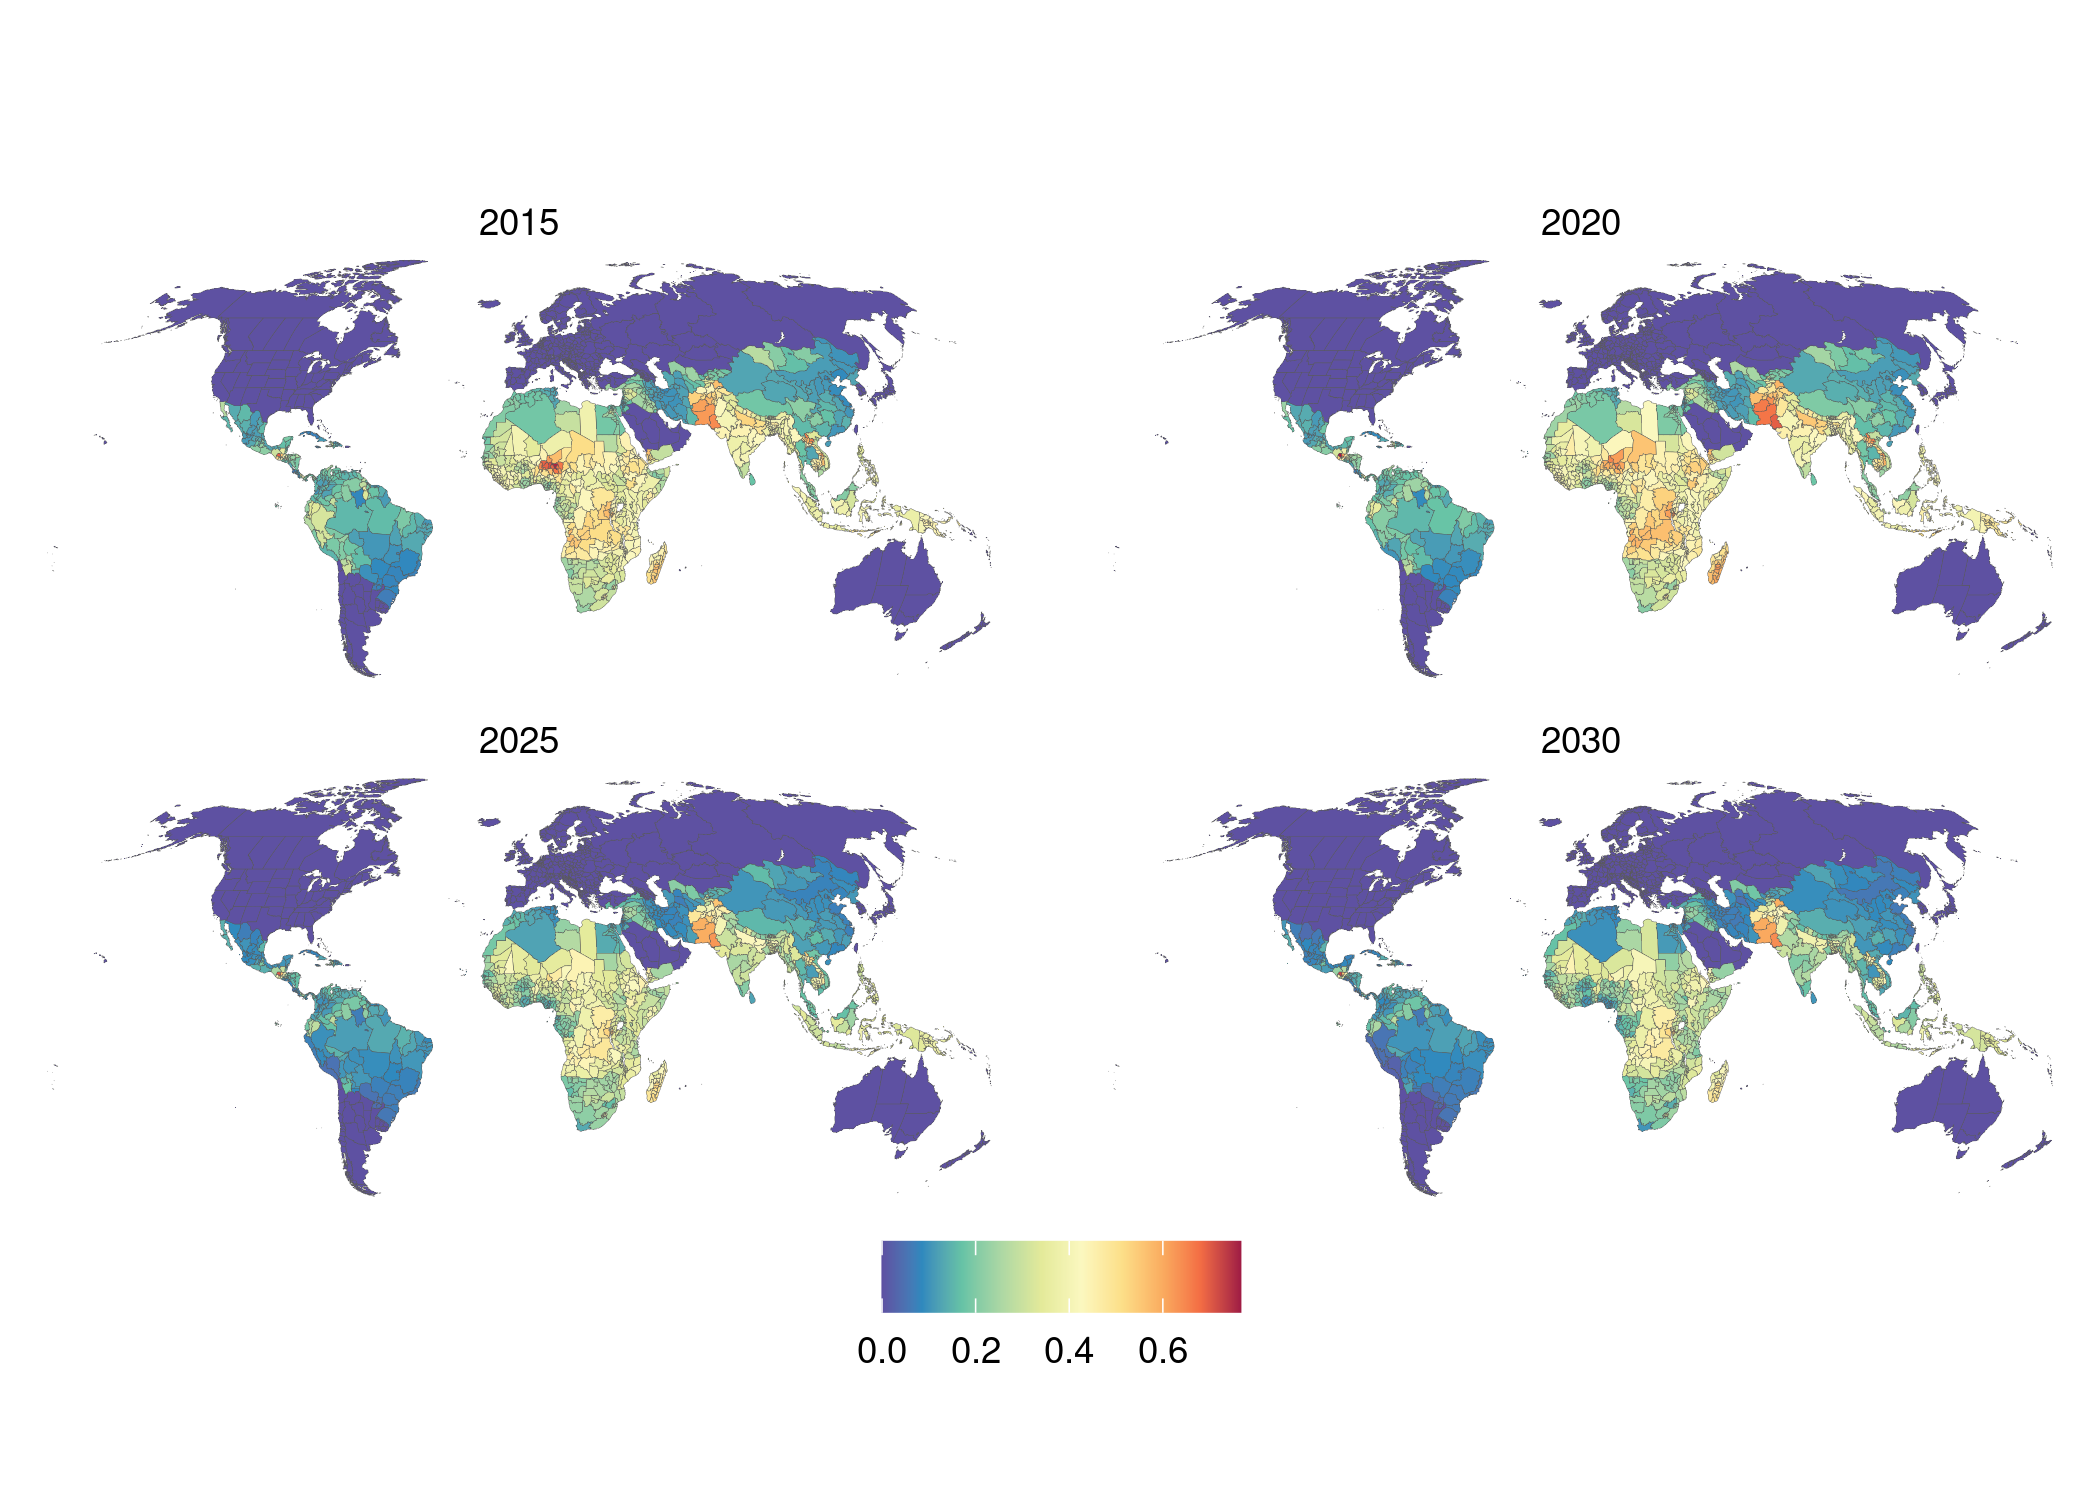
\includegraphics[width=\linewidth]{img/covars/stunting.png}
  \caption{Prevalence of stunting.}
\end{figure}

\subsection{GDP Per Capita}
We estimate global subnational GDP per capita using historic subnational estimates of Gross National Income (GNI) from the Subnational Human Development Database \cite{Smits2019} and forecasts of national GDP within the SSP framework from Dellink et al. \cite{Dellink2017}.  We first use data from the World Bank to estimate the mean country-level ratio of GNI to GDP and adjust the subnational estimates of GNI according to that country-specific ratio.  We then calculate each subnational area's share of country GDP, and then use the AROC method to estimate each subnational area's share of total country GDP.  Based on these trajectories in each subnational areas share of total country GDP, we estimate what each subnational area's share of GDP will be for each year from 2019 to 2030.  We divide that share of GDP by the population of the administrative area, which we had previously estimated.  Thus, national GDP totals are consistent with the projections of Dellink et al., but are disaggregated according to the historic patters of GDP share in the Subnational Human Development Database.

Finally, we used estimates of country-level changes in GDP growth for the years 2020 and 2021 to account for the impact of the coronavirus \citep{prospects2020}.  We then model GDP as resuming its previous growth trajectory based on previously-estimated growth rates from 2022-2030, but growing from an estimate for 2021 that includes the coronavirus shock.

\begin{figure}[H]
  \centering
  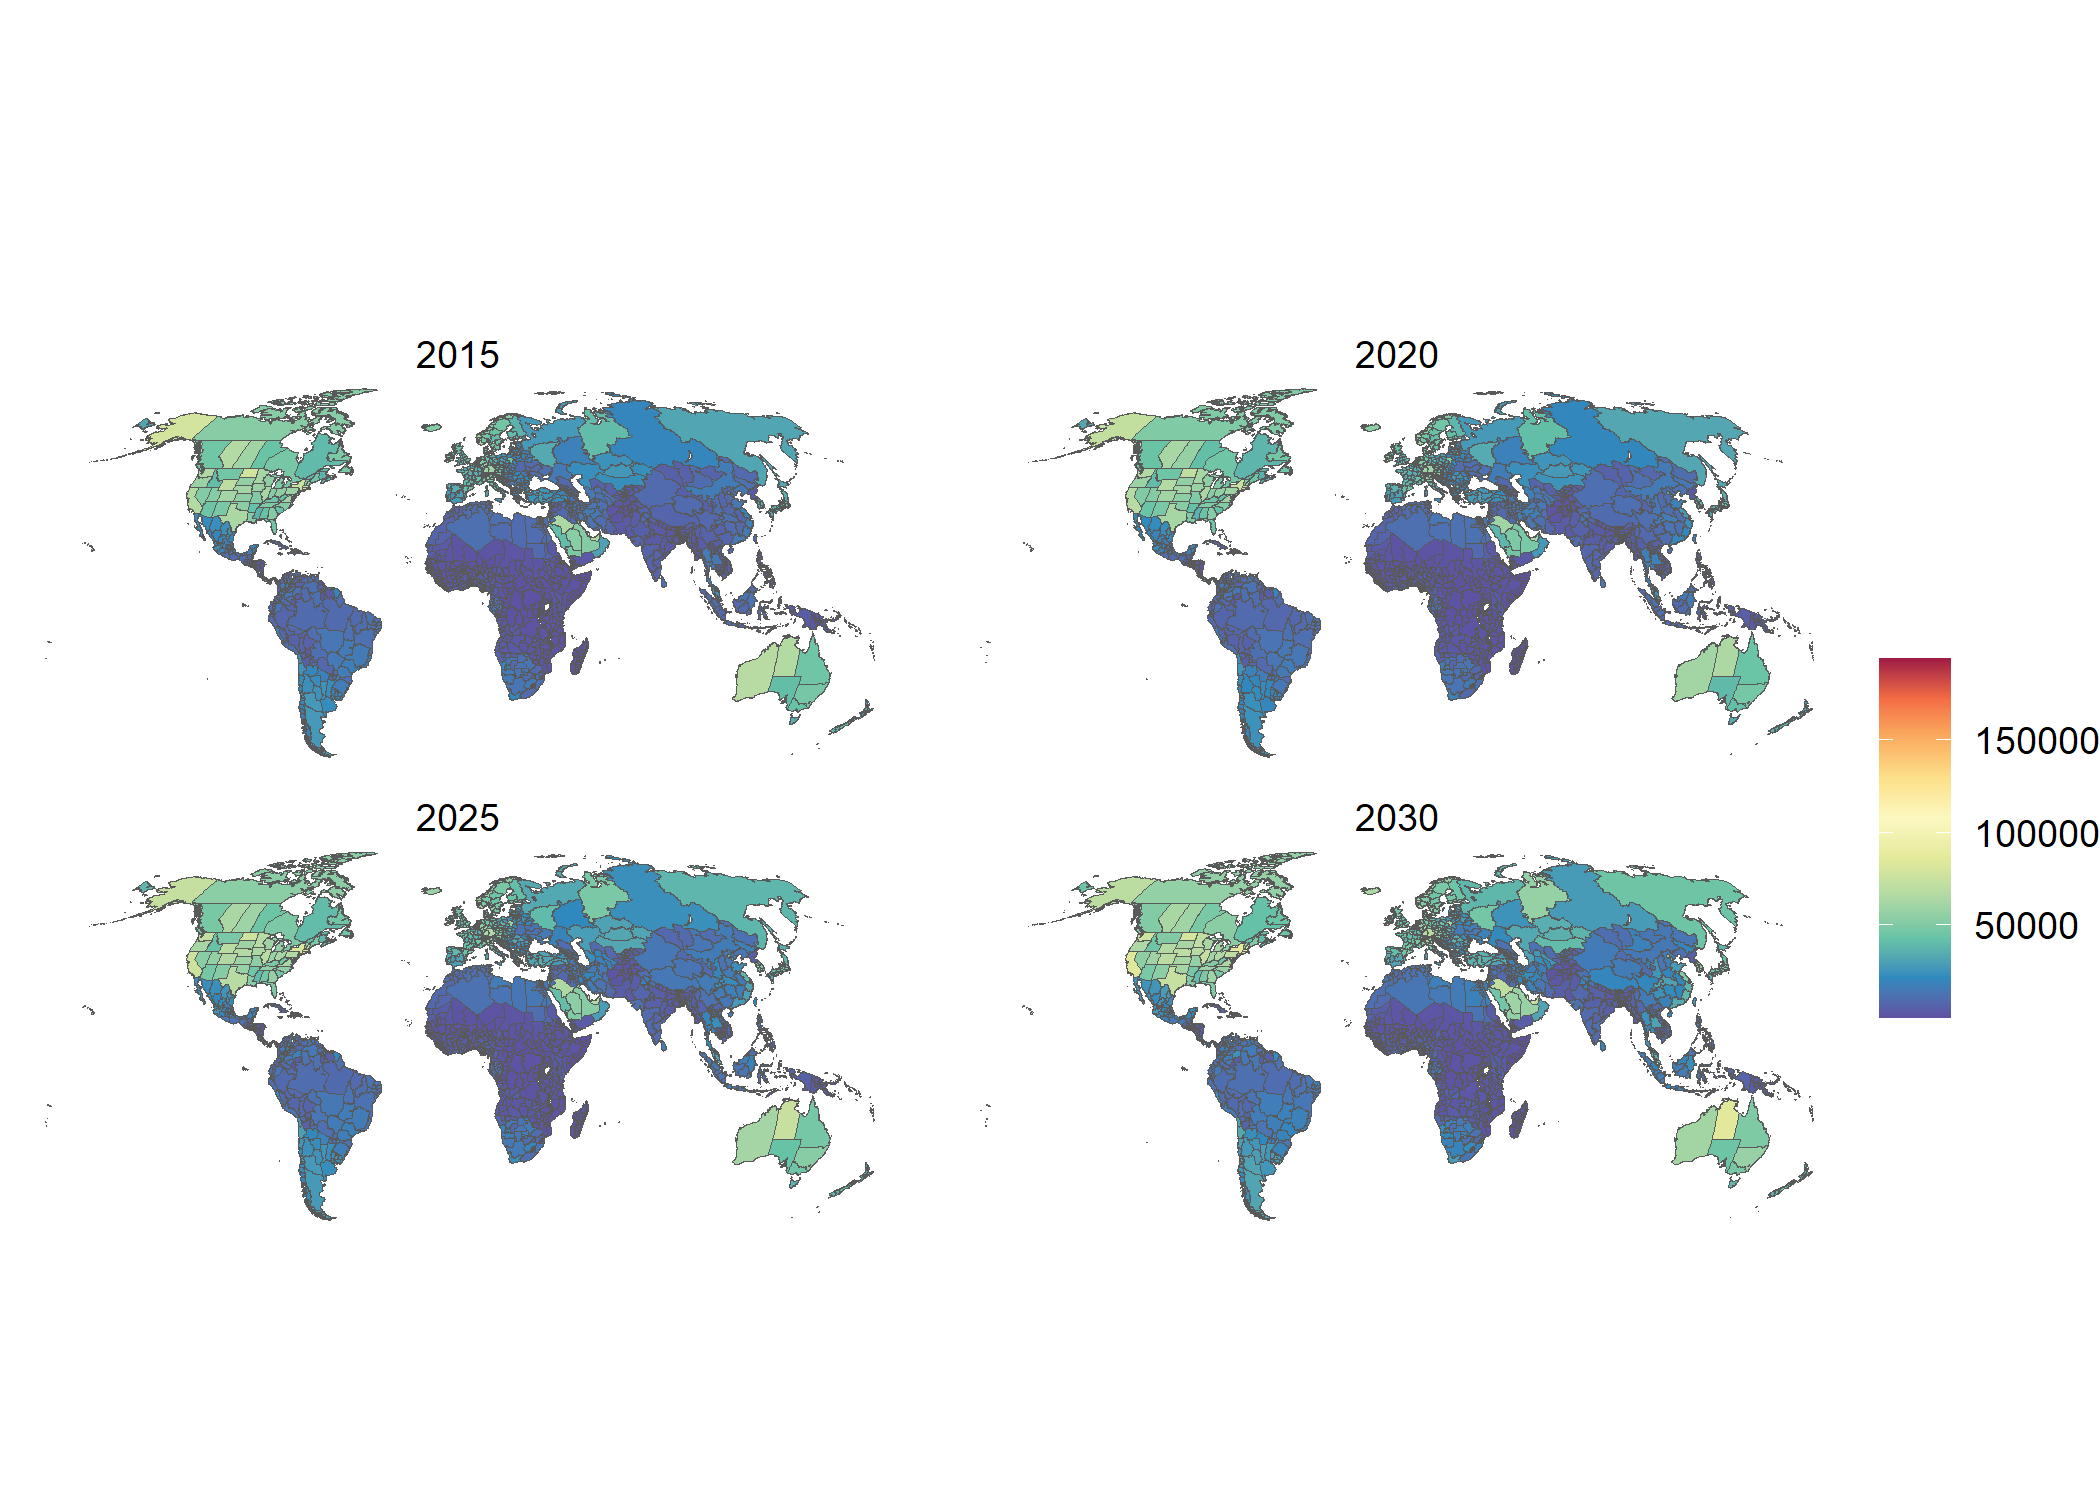
\includegraphics[width=\linewidth]{img/covars/gdp_percap.png}
  \caption{GDP per capita.}
\end{figure}

\subsection{Mean Years of Schooling}
We estimate global subnational mean years of schooling using historic subnational estimates from the Subnational Human Development Database \cite{Smits2019} and forecasts of national mean years of schooling from KC et al. \cite{KC2017}.  Using the historic subnational data, we estimate each subnational administrative area's difference in years of schooling from the national mean, and use this value to disaggregate the future projections to a subnational level.


\begin{figure}[H]
  \centering
  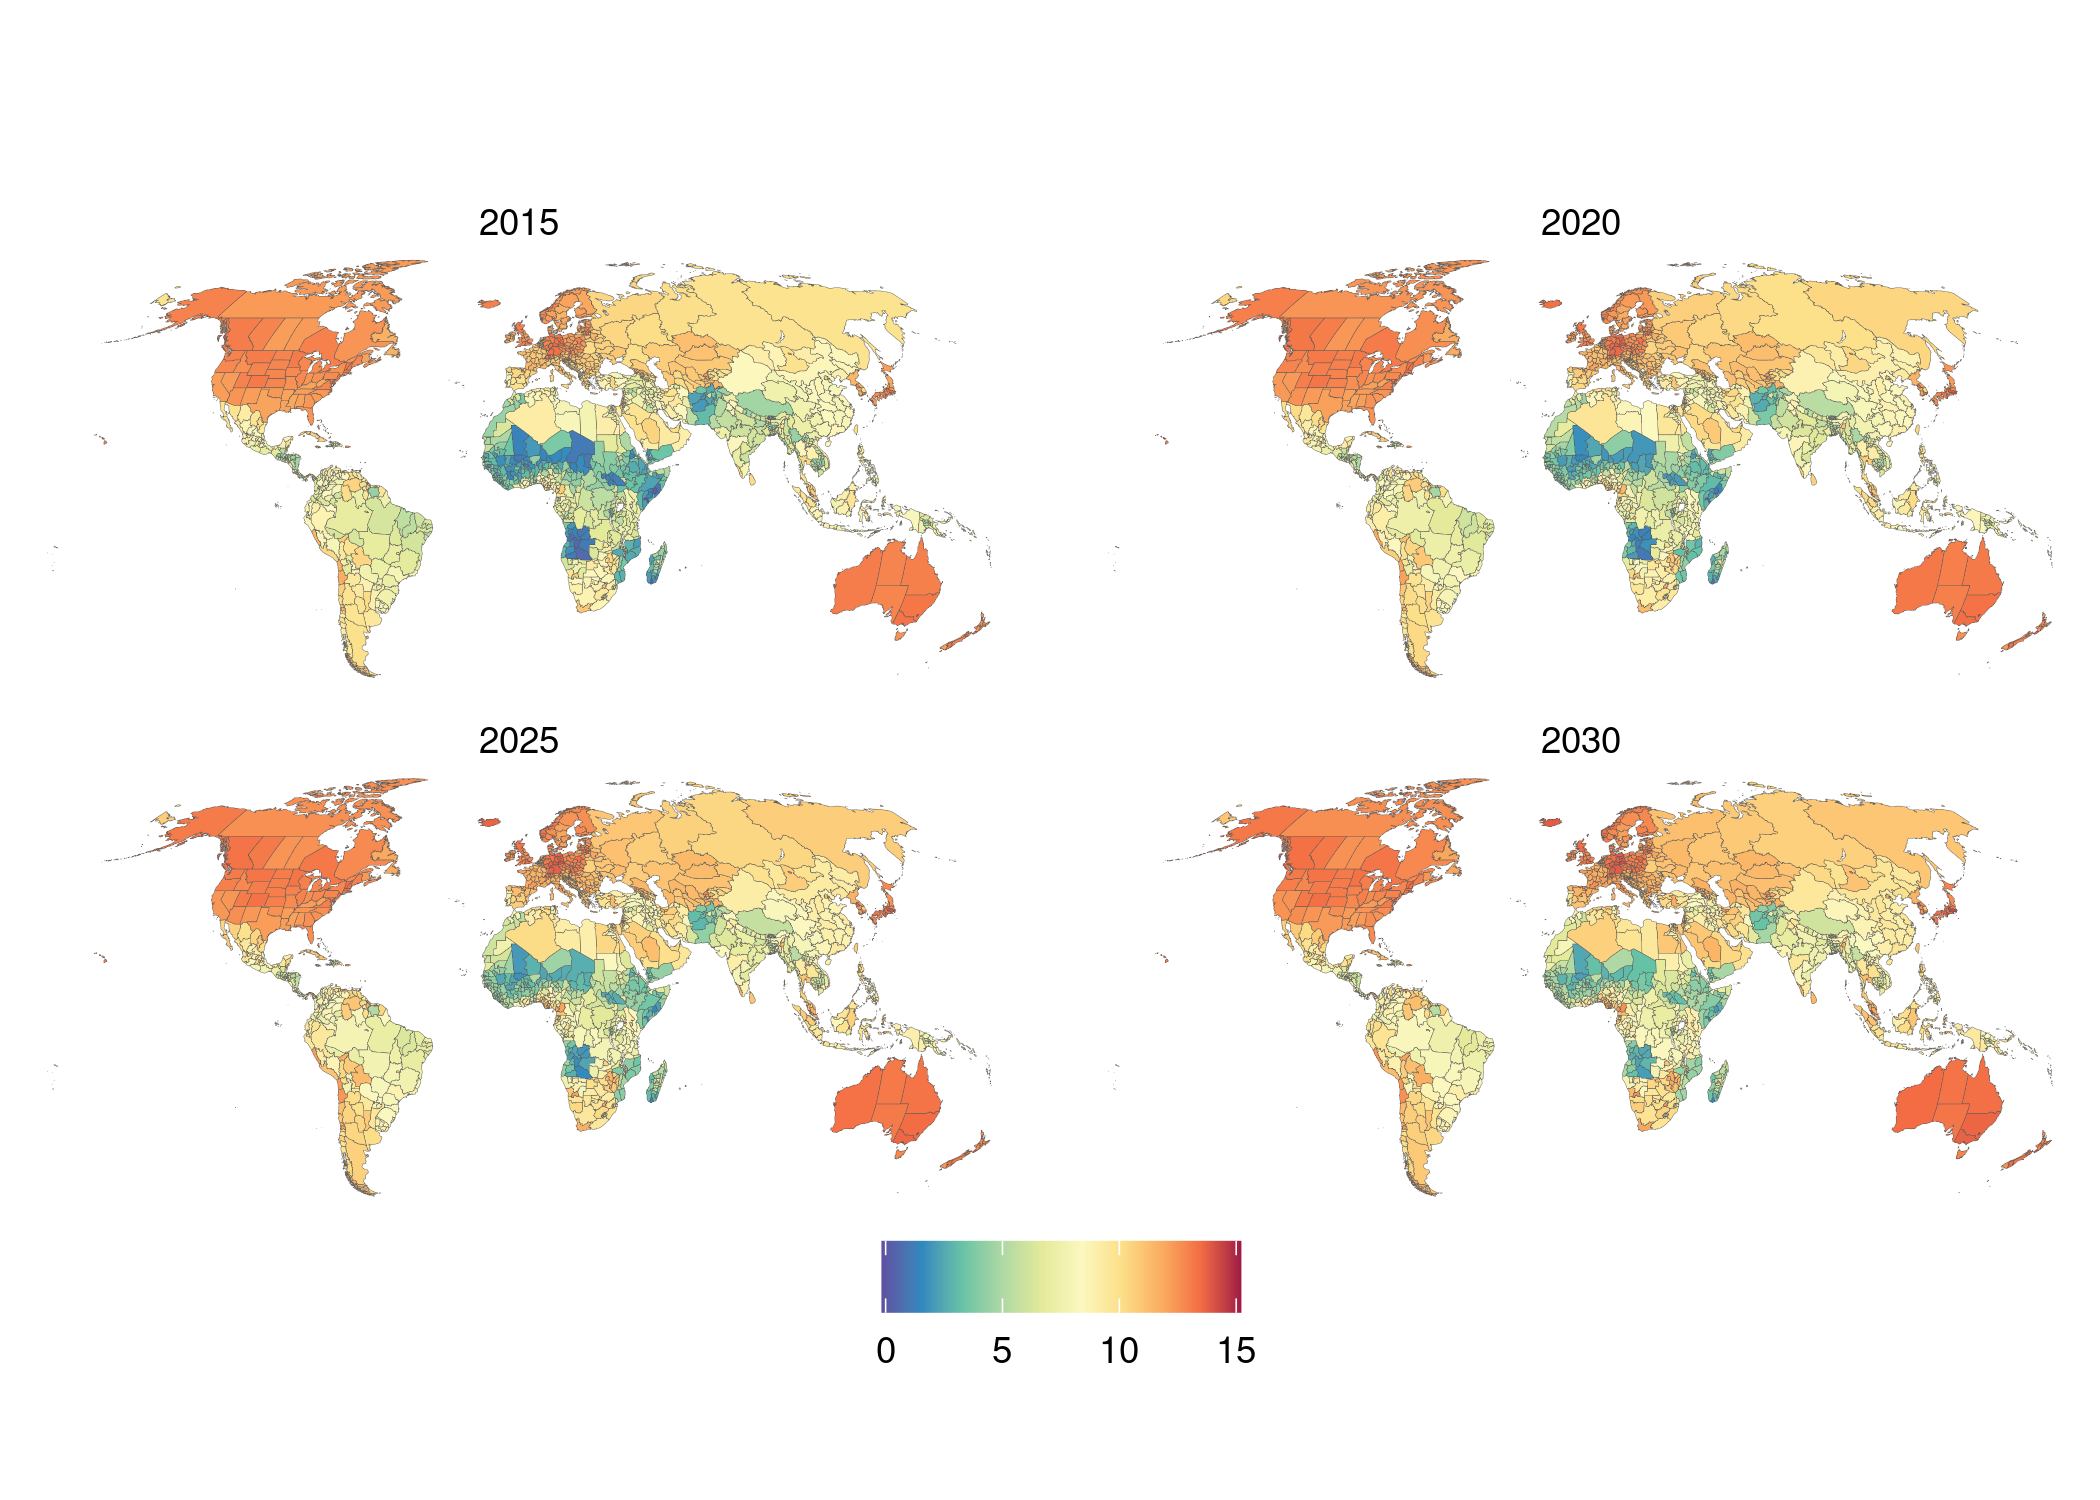
\includegraphics[width=\linewidth]{img/covars/school_mean.png}
  \caption{Mean years of schooling.}
\end{figure}


\subsection{Gini Coefficient}
We use estimates of national income inequality from Rao et al. \citep{Rao2019a}.  These estimates include all years in our analysis, and are not disaggregated to a subnational level.

\begin{figure}[H]
  \centering
  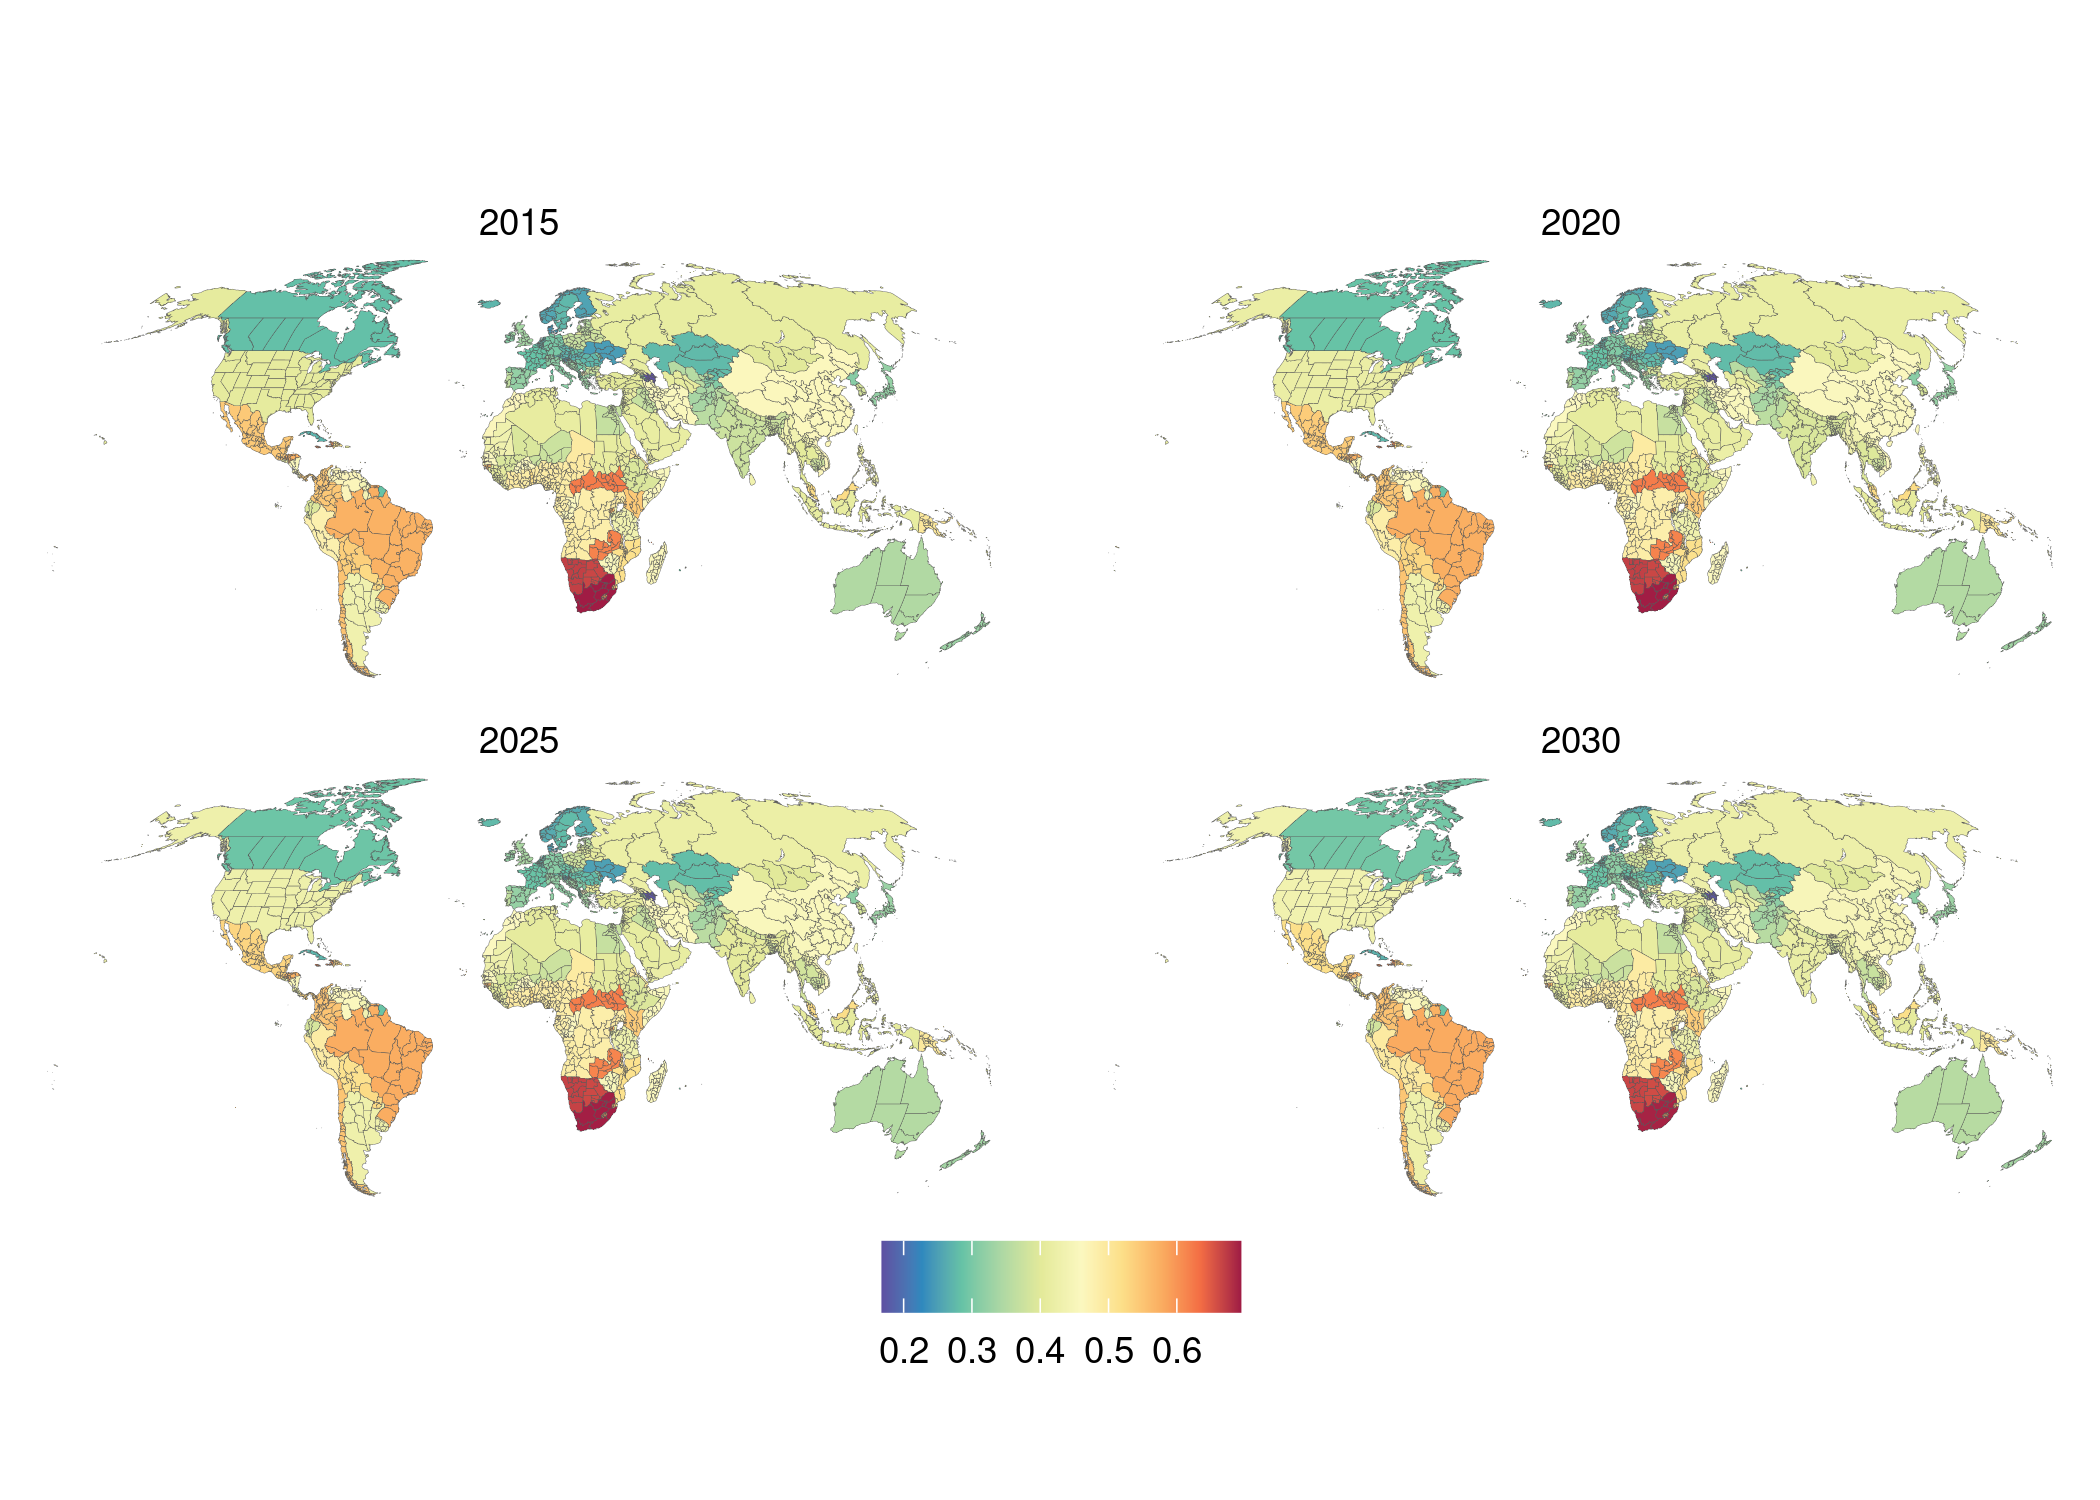
\includegraphics[width=\linewidth]{img/covars/gini.png}
  \caption{Gini Coefficient}
\end{figure}

\subsection{Poverty Headcount Index}
We used estimates of the Poverty Headcount Index for the recent past and future from the World Poverty Clock by the World Data Lab \citep{Cuaresma2018}, updated to include the impact of the coronavirus. In our model we include national level poverty rates at a threshold of \$1.90 which is defined as \textit{extreme} poverty. By using the concept of parameterized Lorenz curves in combination with mean income/consumption and population projections future poverty rates are calculated. For more details on the methodology and information on global and country level poverty check the website \url{worldpoverty.io}.

\begin{figure}[H]
  \centering
  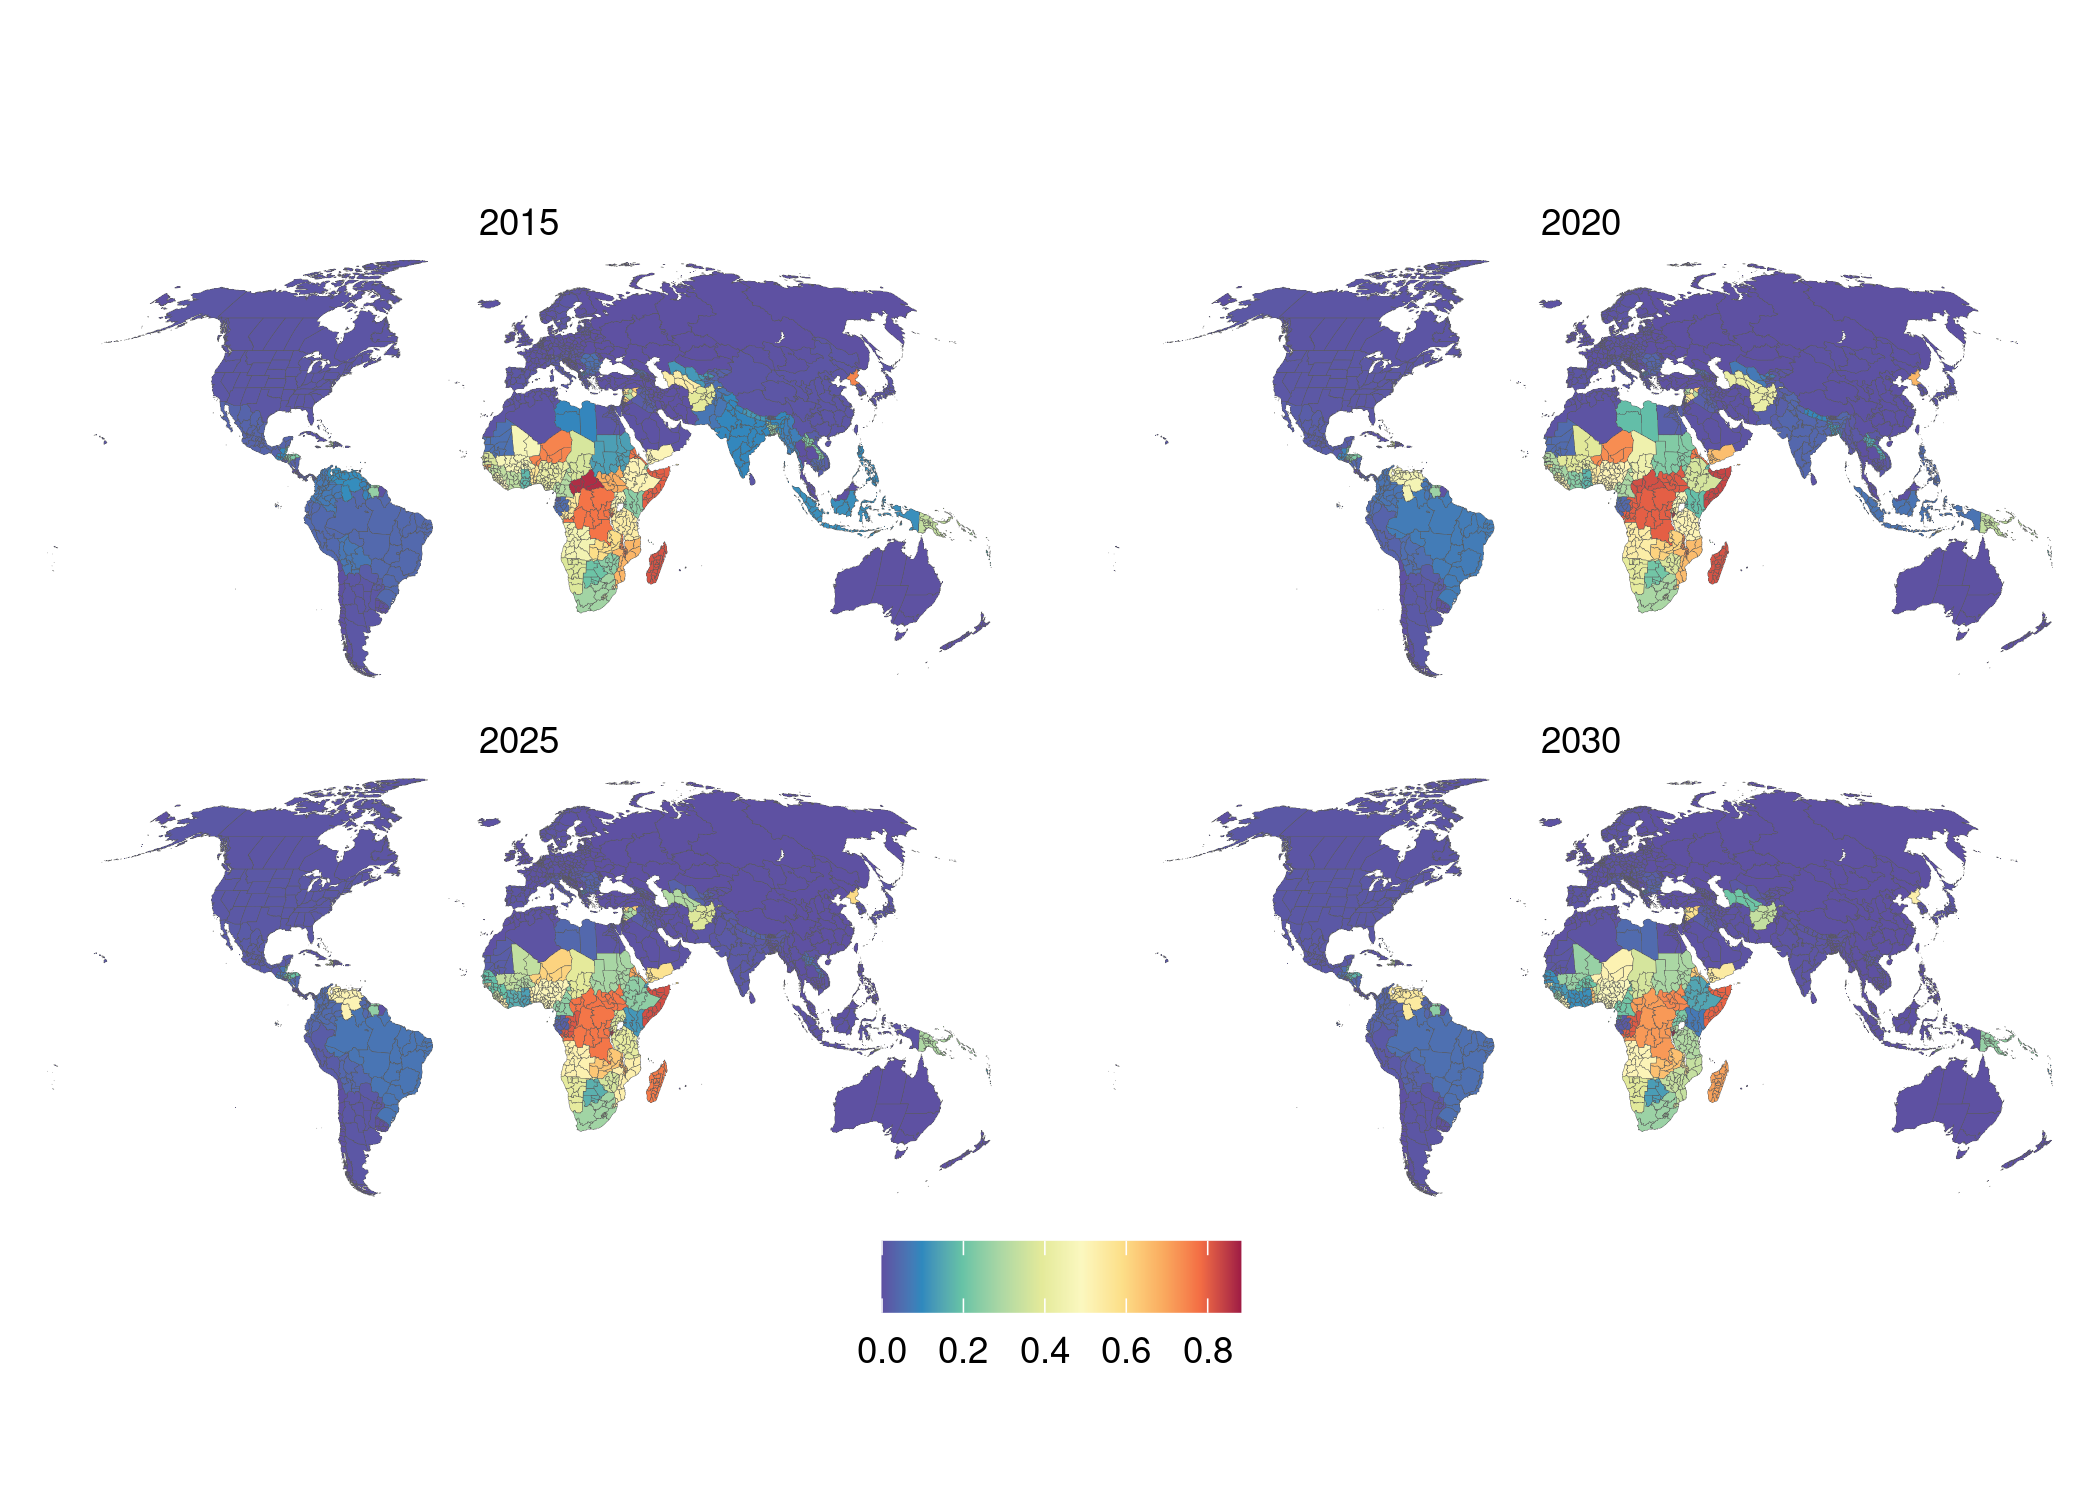
\includegraphics[width=\linewidth]{img/covars/hci.png}
  \caption{Poverty Headcount Index}
\end{figure}


\subsection{Water Scarcity Share}
We used the water scarcity index (WSI) developed by \citep{greve2018global}. The index represents the ratio of the decadal averages in water demand to water supply and it assesses changes in water scarcity on a 0.5 by 0.5 degree global grid.  Based on this index, we estimate the share of people living in areas with less than 1000m\textsuperscript{3} of water available per capita per year. The WSI has been used already to build the water scarcity clock. For more information visit \href{https://worldwater.io/}{worldwater.io}.

\begin{figure}[H]
  \centering
  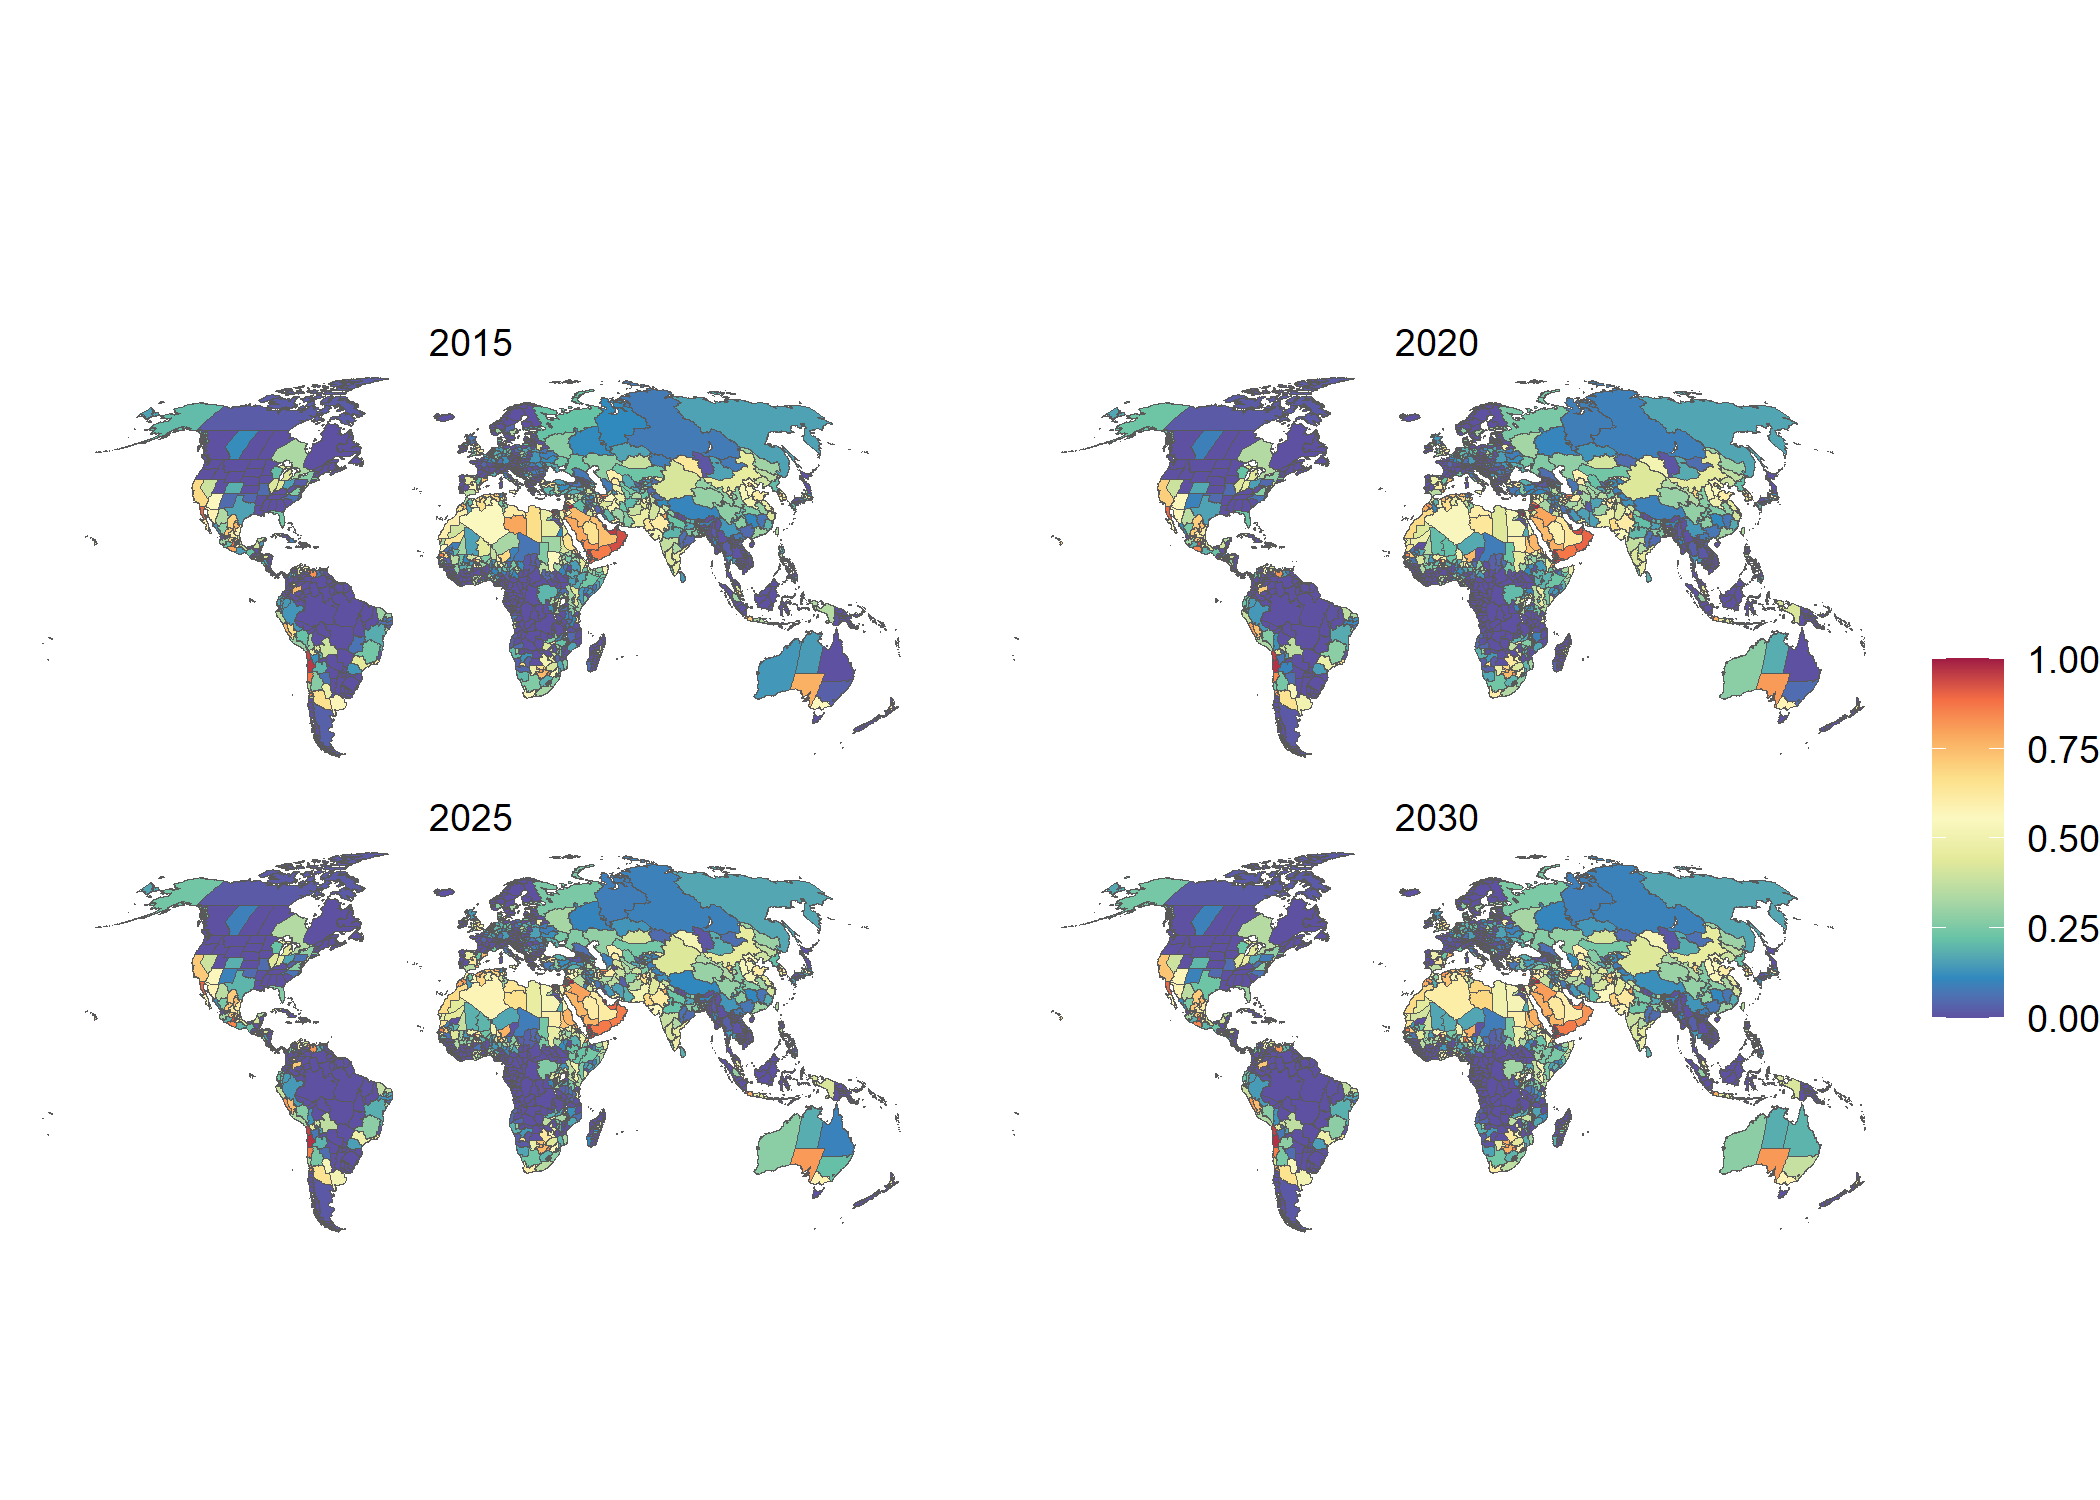
\includegraphics[width=\linewidth]{img/covars/ws_share.png}
  \caption{Water Scarcity Share}
\end{figure}


\subsection{Mean Annual Precipitation}
For mean annual precipitation, we use data for the years 2010 to 2019 from the TerraClimate dataset \citep{abatzoglou2018terraclimate}, summarized to each subnational area.  For data for the years 2020-2030, we use models from the Inter-Sectoral Model Intercomparison Project \citep{warszawski2014inter}.  Specifically, we use an ensemble of bias-corrected projections under representative concentration pathway (RCP) 6.0, taking the mean of the ensemble.

\begin{figure}[H]
  \centering
  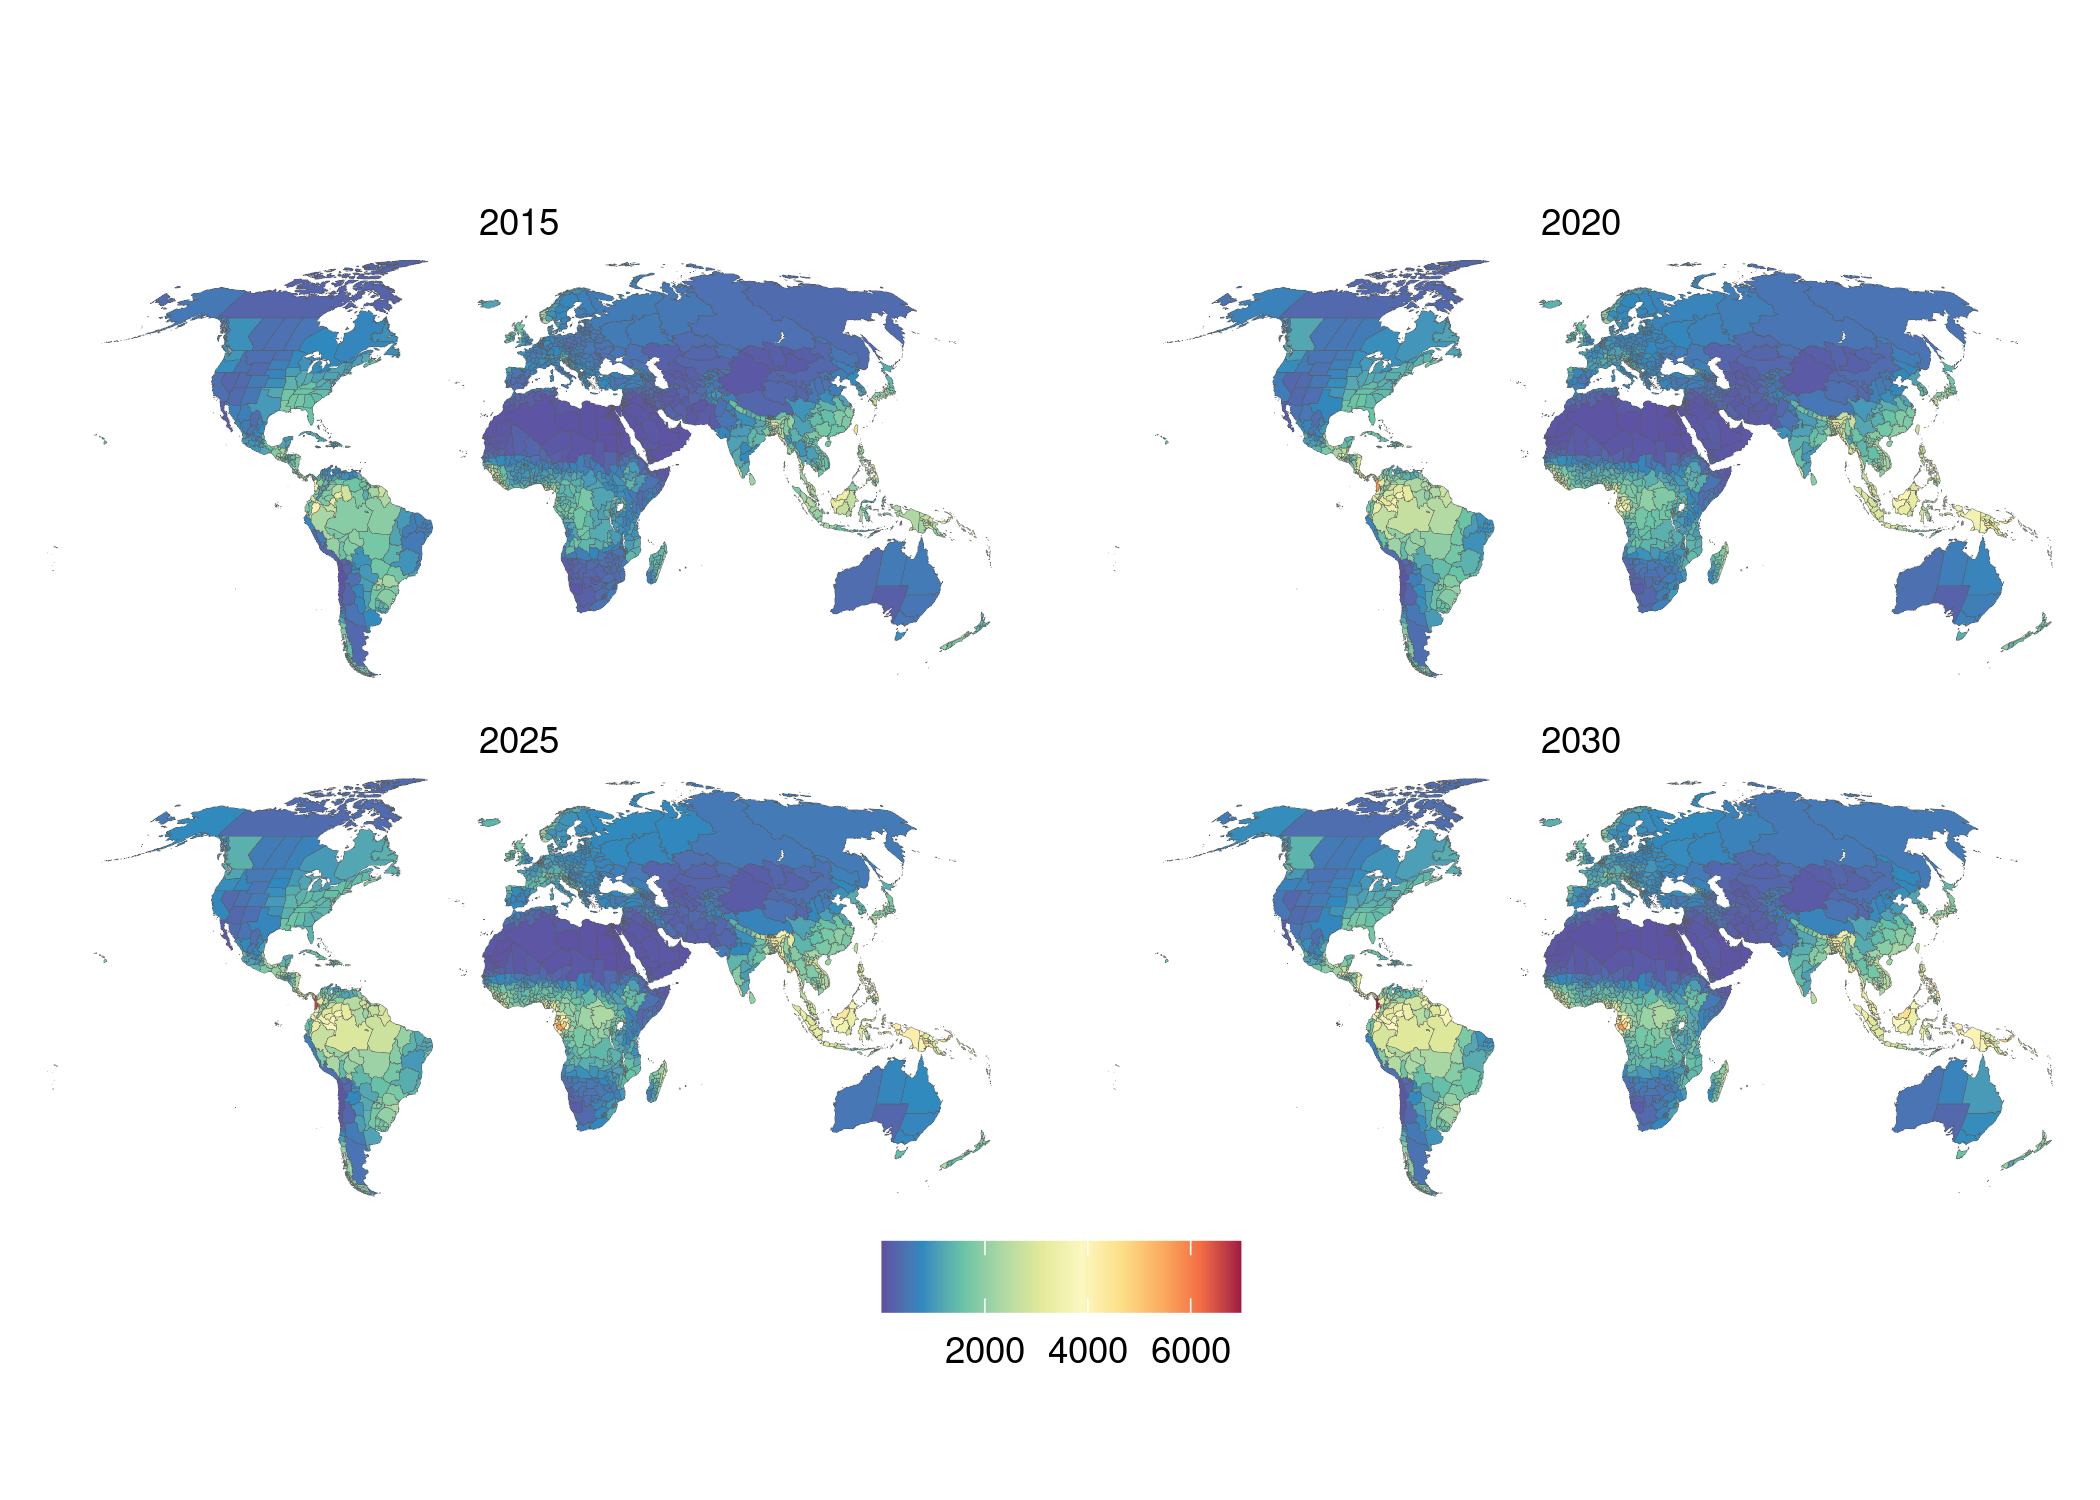
\includegraphics[width=\linewidth]{img/covars/precip.png}
  \caption{Mean annual precipitation}
\end{figure}

\subsection{Mean Temperature}
For mean temperature, we used the same datasets that we'd used for precipitation, as each of those datasets included both temperature in addition to precipitation.

\begin{figure}[H]
  \centering
  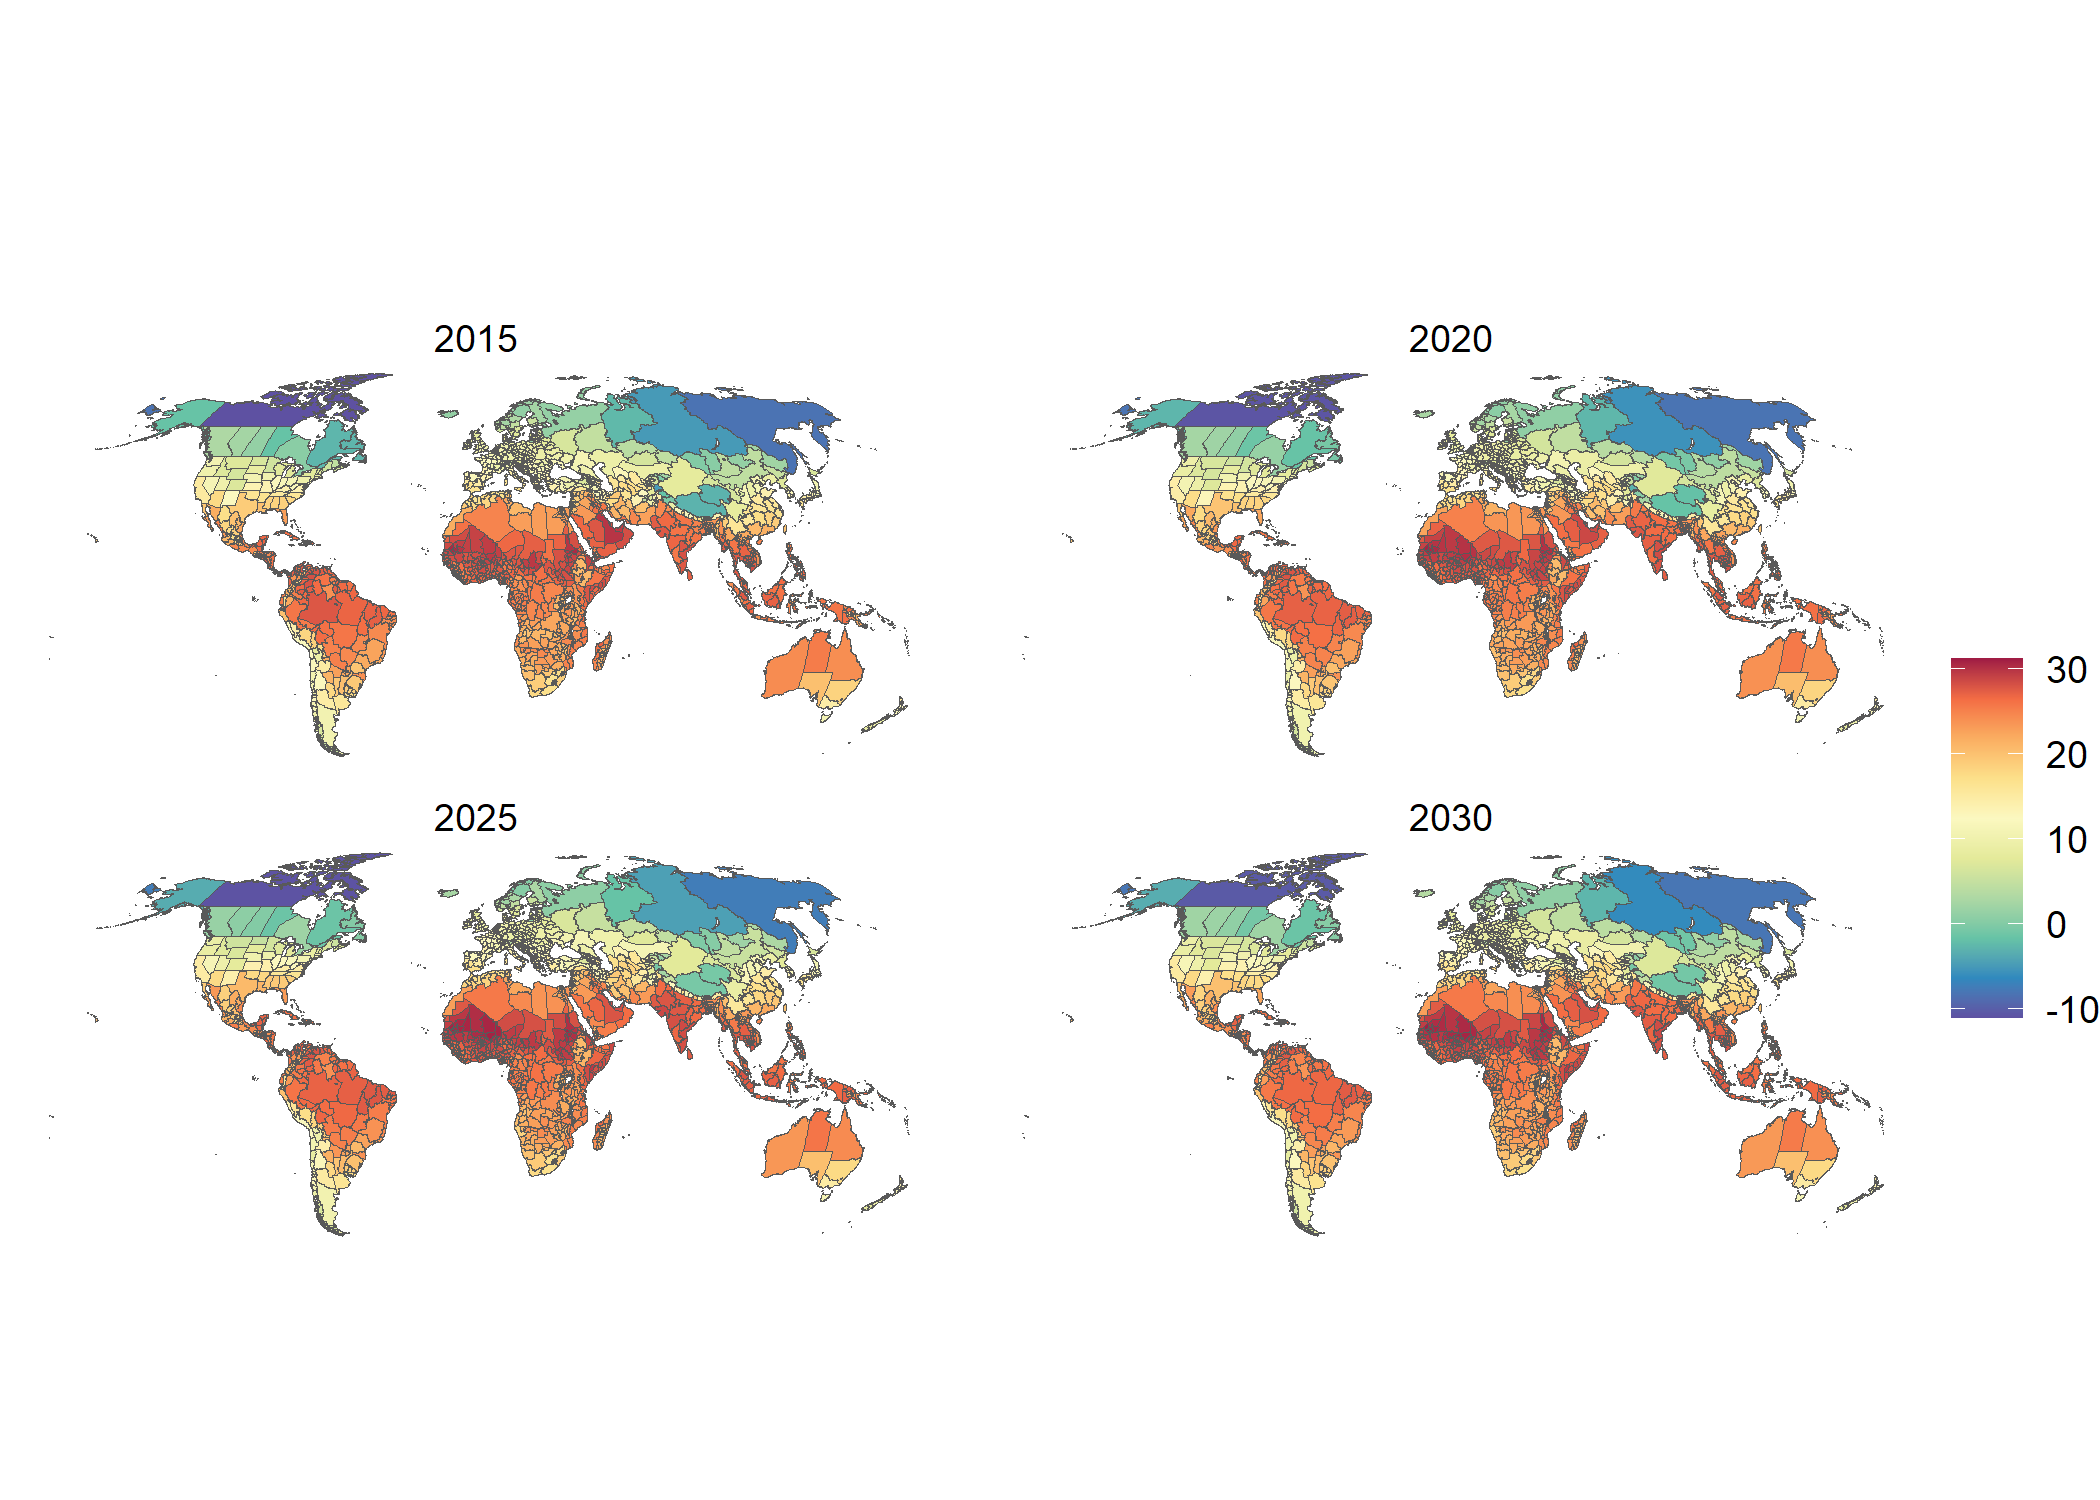
\includegraphics[width=\linewidth]{img/covars/tave.png}
  \caption{Mean temperature (Celsius)}
\end{figure}

\subsection{Topographic Ruggedness}
As a measure of accessibility, we include the mean topographic ruggedness of each subnational area.  We first used a gridded dataset of elevation from the USGS \cite{USGS1996} and calculated the index at each grid cell using the methodology from Riley et al. \citep{Riley1999}.  We then summarized the values of all the grid cells within each administrative area.  Because this variable does not change over time, it is constant across all years in the model.

\begin{figure}[H]
  \centering
  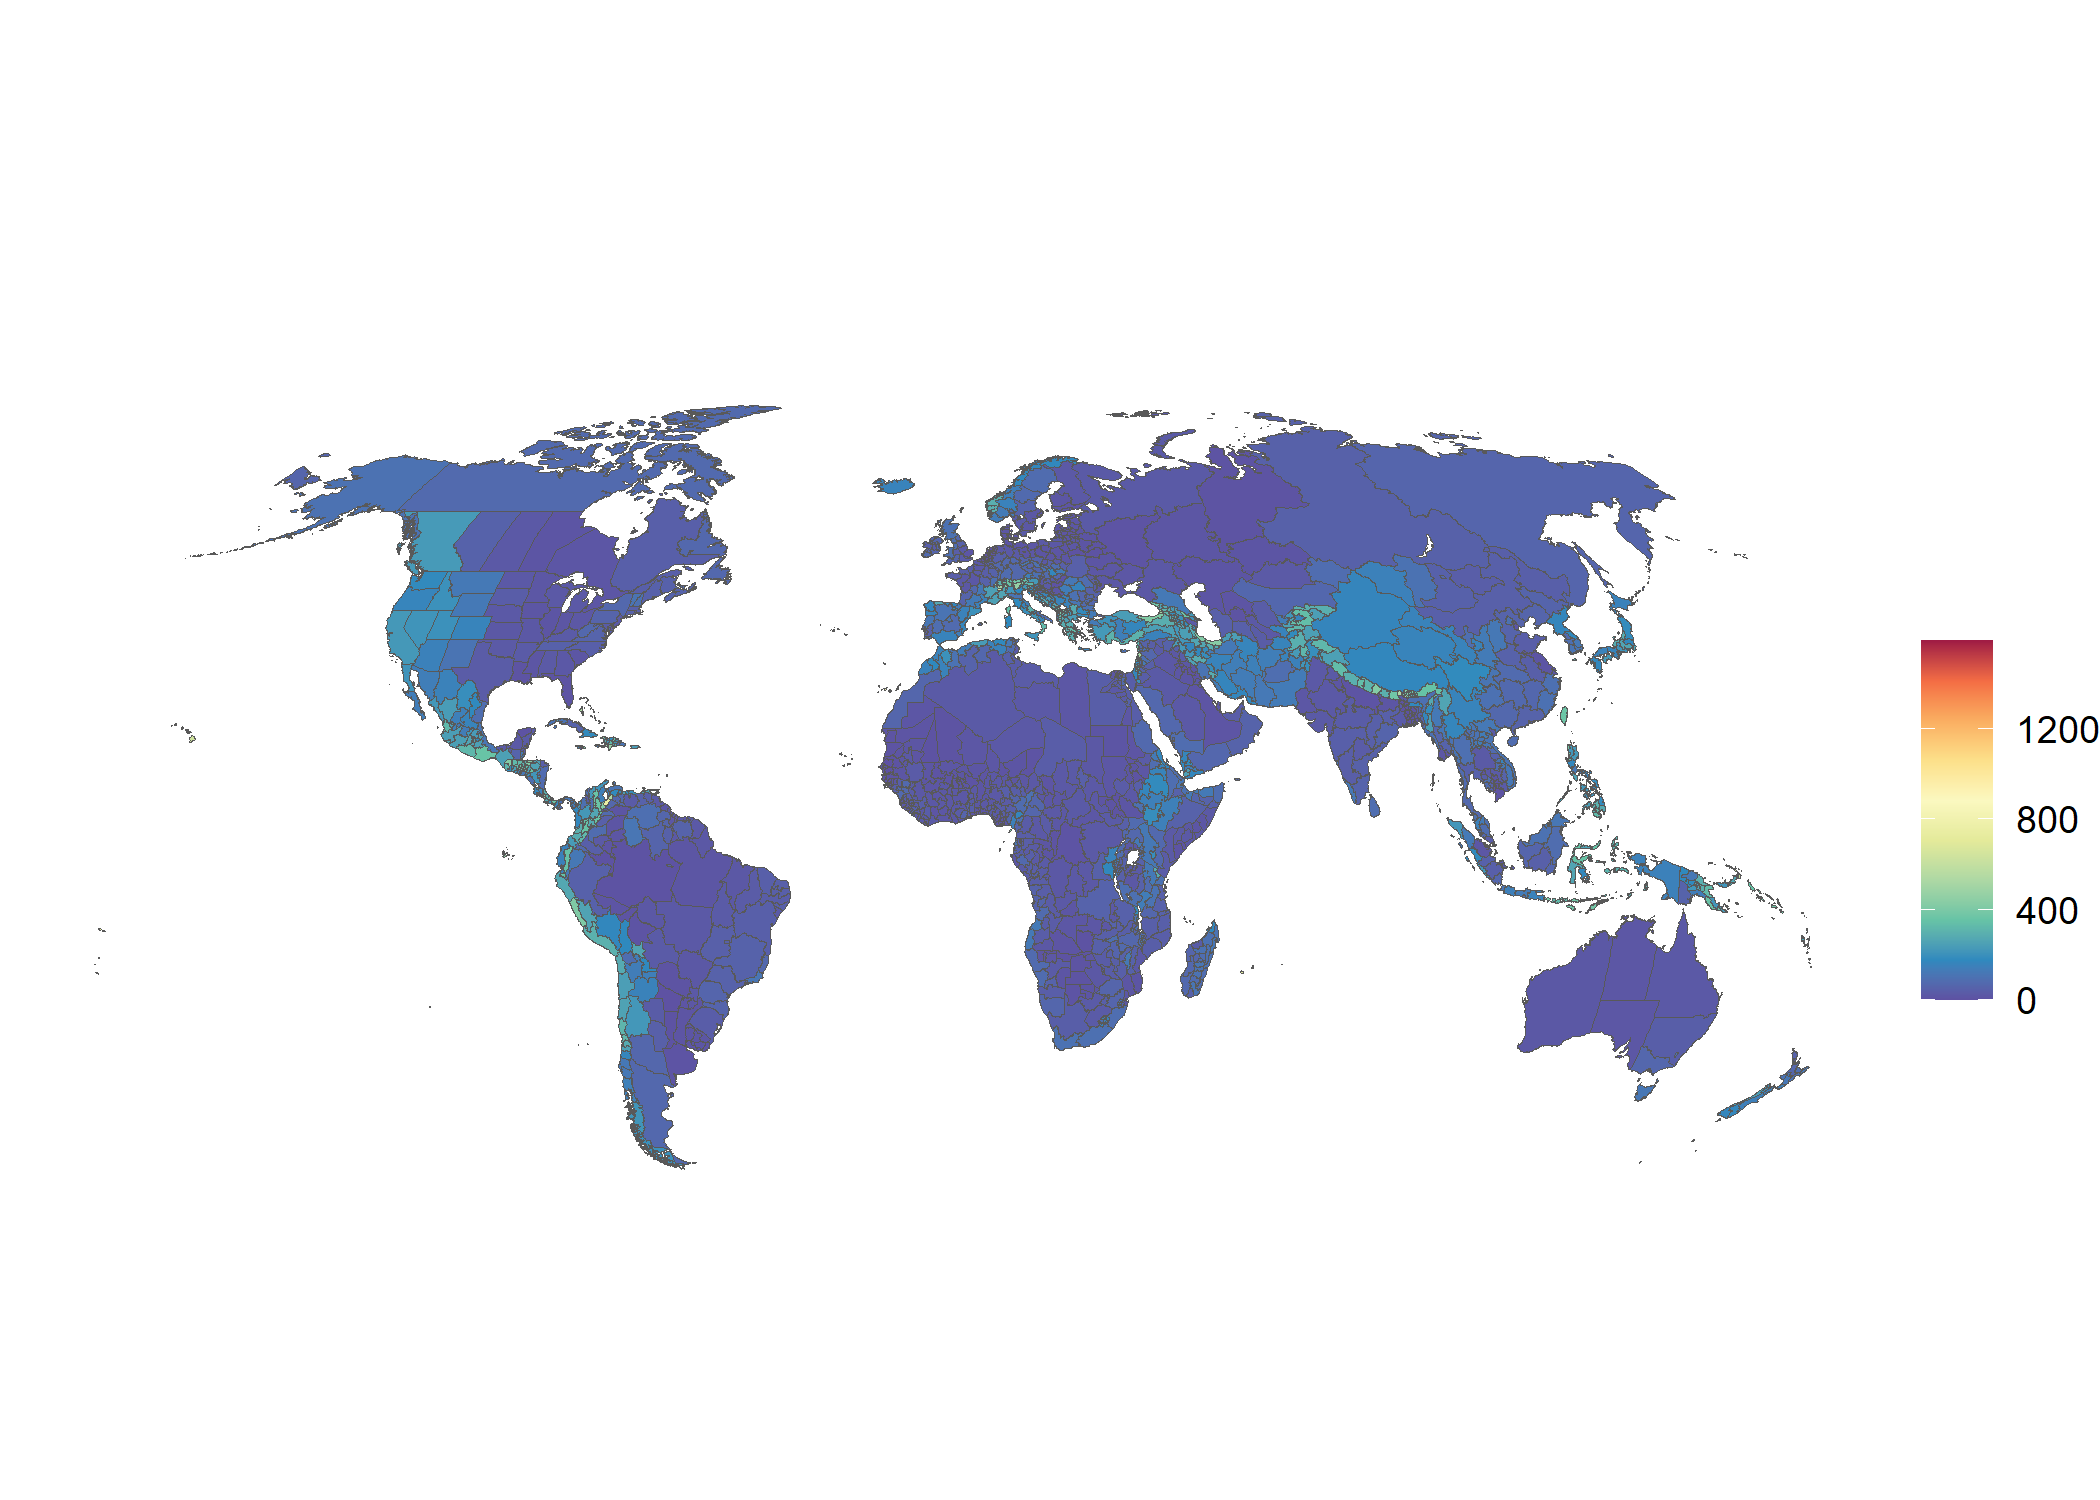
\includegraphics[width=\linewidth]{img/covars/ruggedness.png}
  \caption{Topographic ruggedness}
\end{figure}

\subsection{Malaria (\textit{P. falciparum}) Mortality Rate}
We used data from \textit{The Lancet} to estimate the mortality (deaths per 100,000 population per year) due to Malaria \citep{Weiss2019}, taking the average pixel values within each subnational administrative area.  We then estimated future malaria mortality based on AROC method.

\begin{figure}[H]
  \centering
  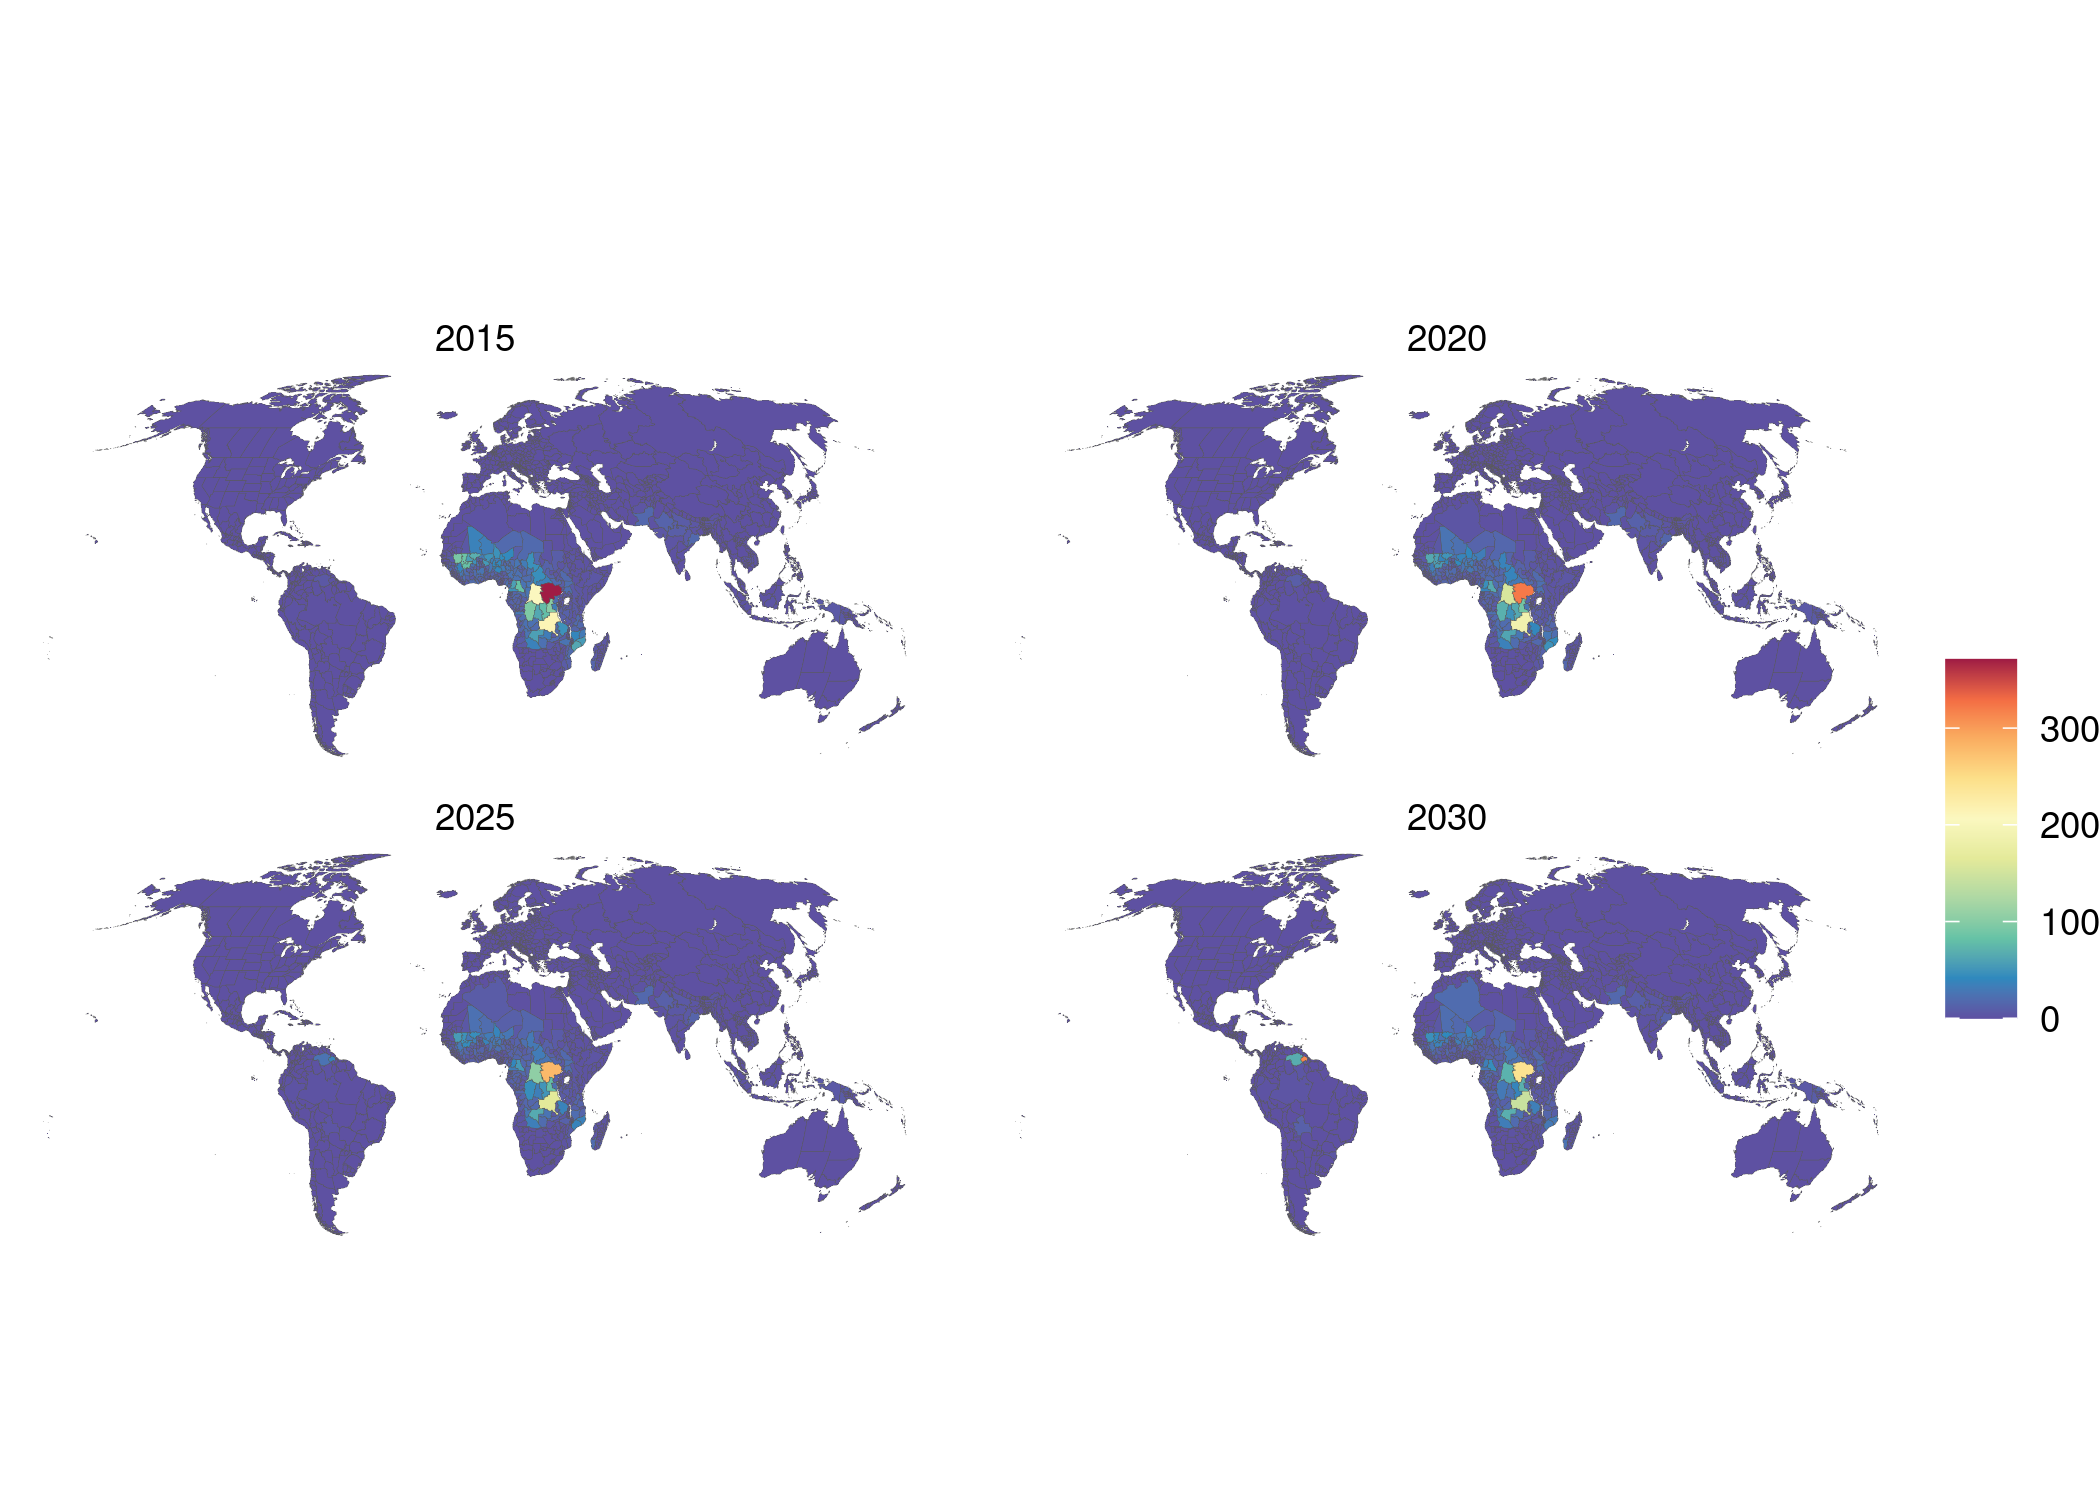
\includegraphics[width=\linewidth]{img/covars/mal_falciparum.png}
  \caption{Rate of mortality due to \textit{P. falciparum} Malaria}
\end{figure}

\section{Description, Implementation and Validation of the RF regression model}

The RF regression is a machine learning method based on the creation of a large number of decision trees. By taking an ensemble of decision tree models, random forests introduce more variance and balance out the bias that is common to single decision trees \citep{friedman2001elements}.  For each of the decision trees in a random forest model, observations are selected at random with replacement, a method known as bootstrap aggregating, or bagging, and features are area also selected at random.

For implementation we use the R-package \texttt{randomForestSRC} by Ishwaran and Kogalur \citep{ishwaran2019randomforestsrc}. Specifically, we apply the functions \texttt{tune.rfsrc()} to find the optimal combination of hyperparamters and the function \texttt{rfsrc()} to perform the RF regression models. After predicting rates of moderate-to-severe and severe food insecurity we plot the modeled vs. observed rates and calculated the MSE and ${R}^2$ (See Fig. \ref{fig:rf_in-sample} and Fig. \ref{fig:rf_out-sample}) for both models. Additionally, we use the function \texttt{vimp()} to gain insights into the development of the error rates with increasing numbers of trees (See Fig. \ref{fig:rf_error}) and the importance of individual variables (See Fig. \ref{fig:rf_vimp}).

%STEP-BY-STEP: LOGIT TRANSFORM, TUNE, MODEL, PREDICT, VALIDATE

To ensure that predicted rates are bounded by 0 and 1 we conduct a logit transformation of the dependent variable and inverse logit transformation of the predictions. 
%MAYBE STATE THIS SOMEWHERE ELSE, NOT SURE WHERE

\begin{figure}[H]
  \centering
  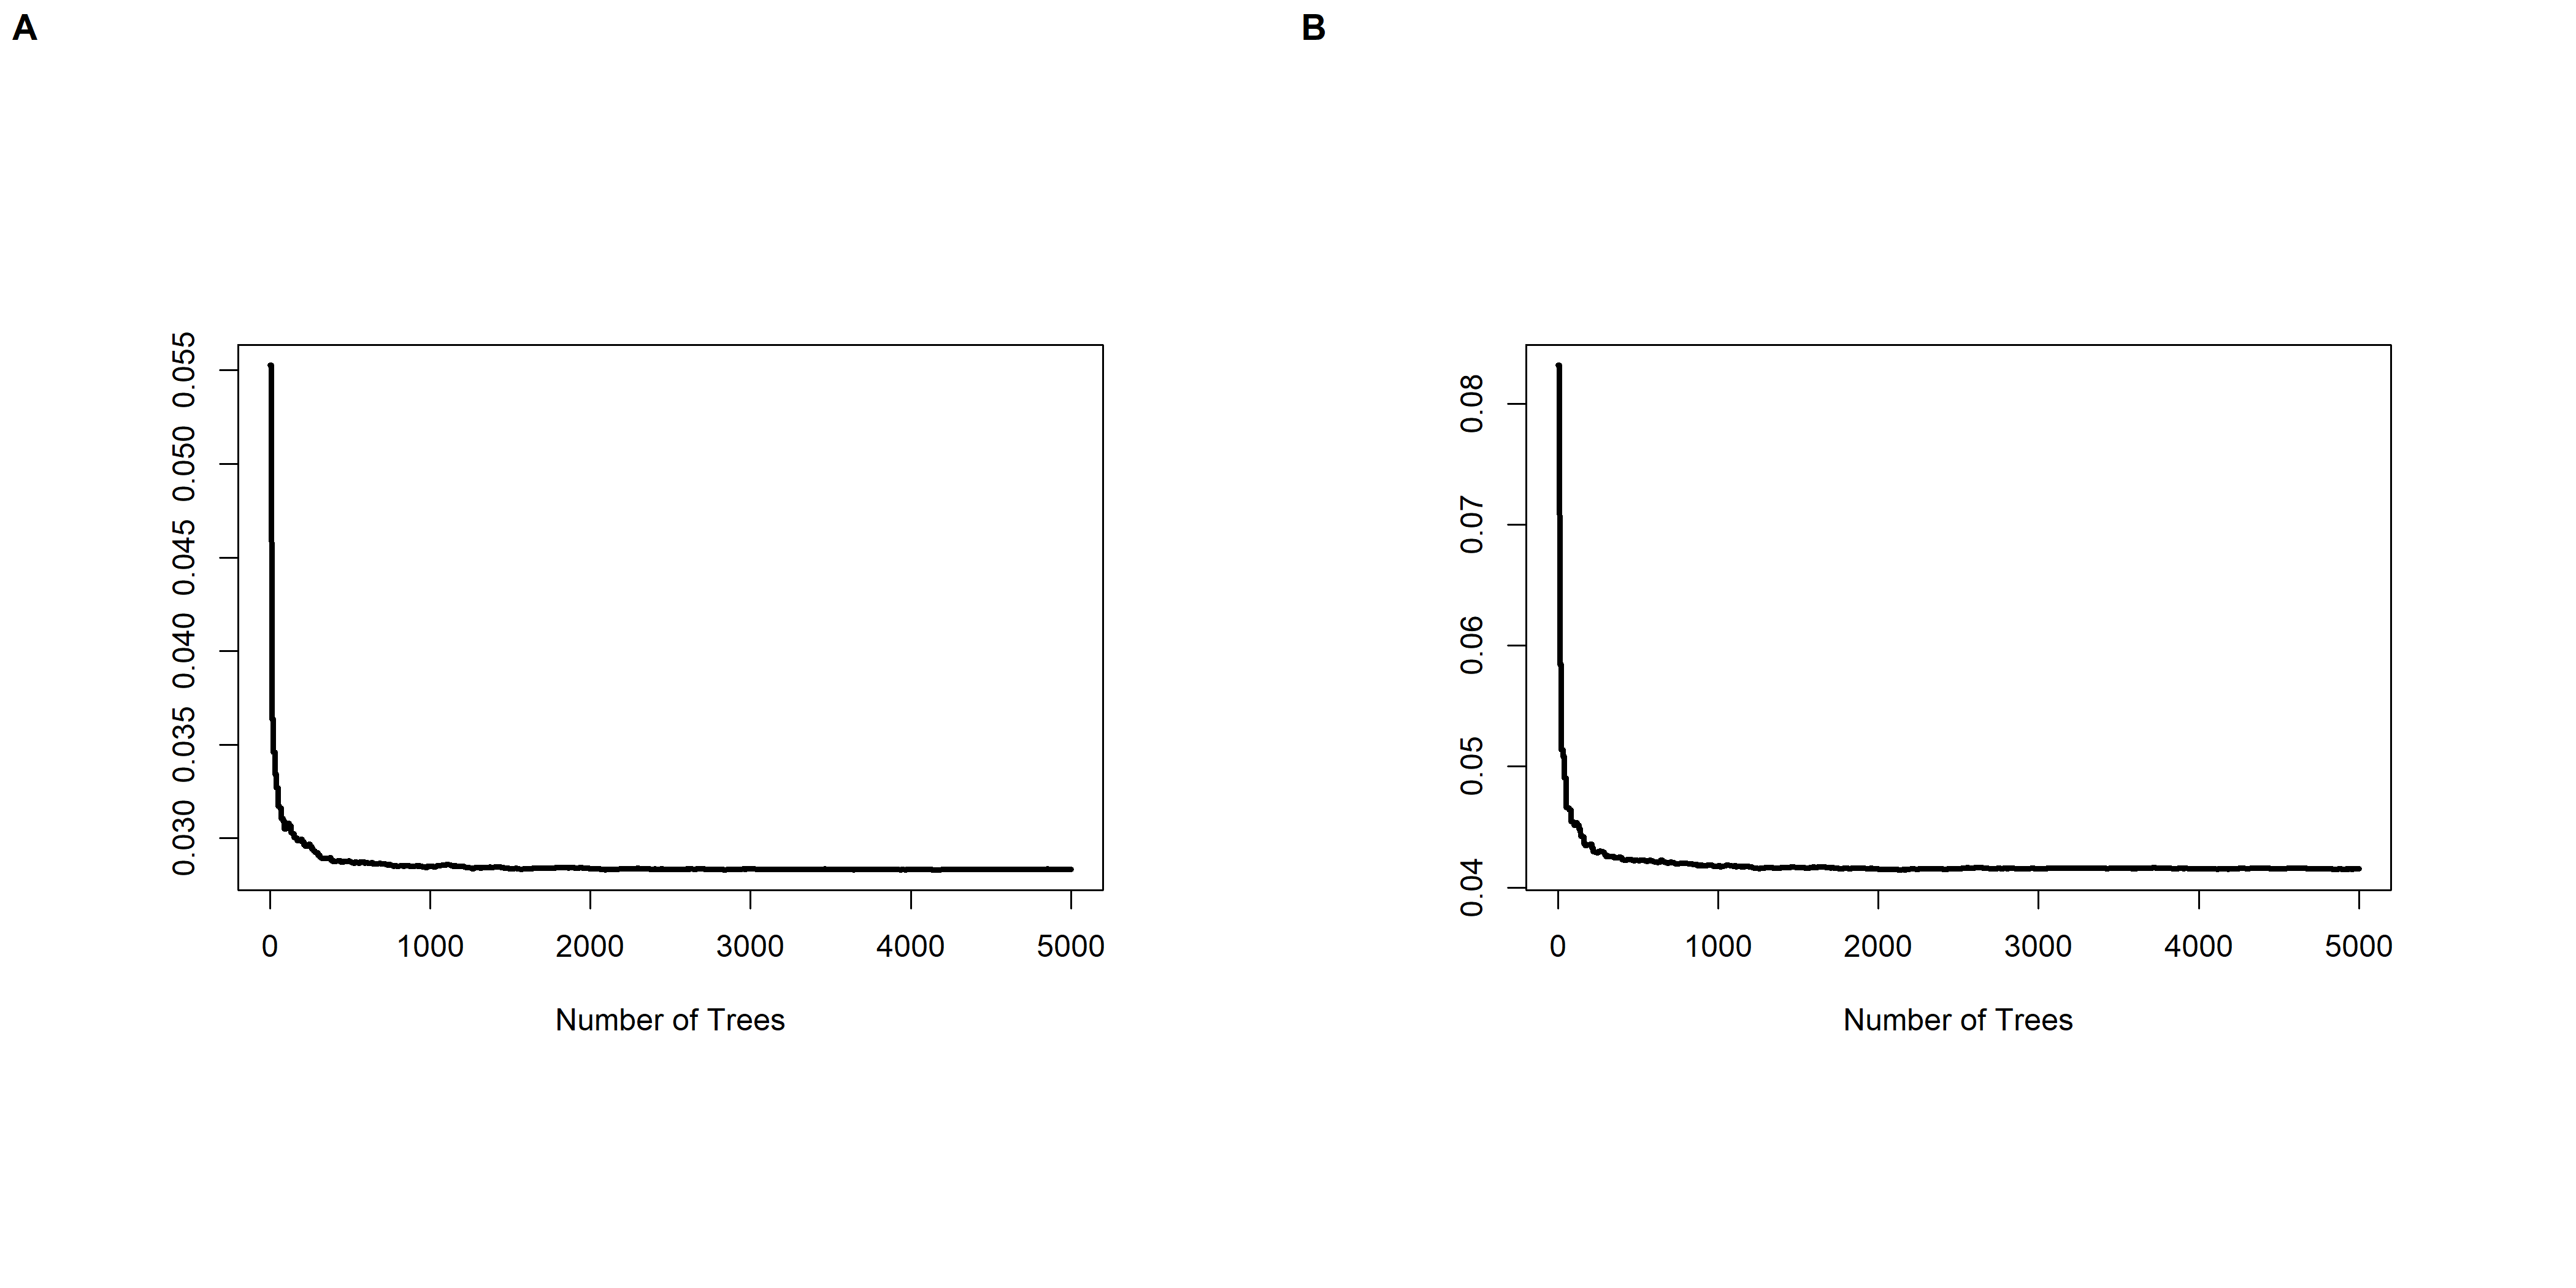
\includegraphics[width=\linewidth]{img/model/error_rf.png}
  \caption{Error Rate of the RF regression model. Panel (A) shows the Moderate-to-Severe model and Panel (B) shows the Severe model.}
  \label{fig:rf_error}
\end{figure}

%HERE A FEW SENTENCES ON THE NUMBER OF TREES WITH LINK TO NEXT PARAGRAPH

In addition to the parameter that describes the number of trees to be created, two other important hyperparameters must be tuned. In the function \texttt{tune.rfsrc()} these parameters are called \texttt{mtry} and \texttt{nodesize}. \texttt{mtry} describes the number of variables randomly selected as candidates for splitting a node and \texttt{nodesize} describes the average number of observations in a leaf node. The optimal pair of hyperparamters is found by trying different combinations and choosing the one with the smallest out-of-bag (OOB) error.

%EXPLAIN THE OOB ERROR HERE?

The function \texttt{tune.rfsrc()} does exactly that and returns optimal values for \texttt{mtry} and \texttt{nodesize}. We applied this function on both, the moderate-to-severe and the severe model. For the moderate-to-severe model the optimal combination is \texttt{mtry} = 12 and \texttt{nodesize} = 1 and for the severe model we found \texttt{mtry} = 10 and \texttt{nodesize} = 2 to be optimal.

%STATE FUNCTION ARGUMENTS HERE?

\begin{figure}[H]
  \centering
  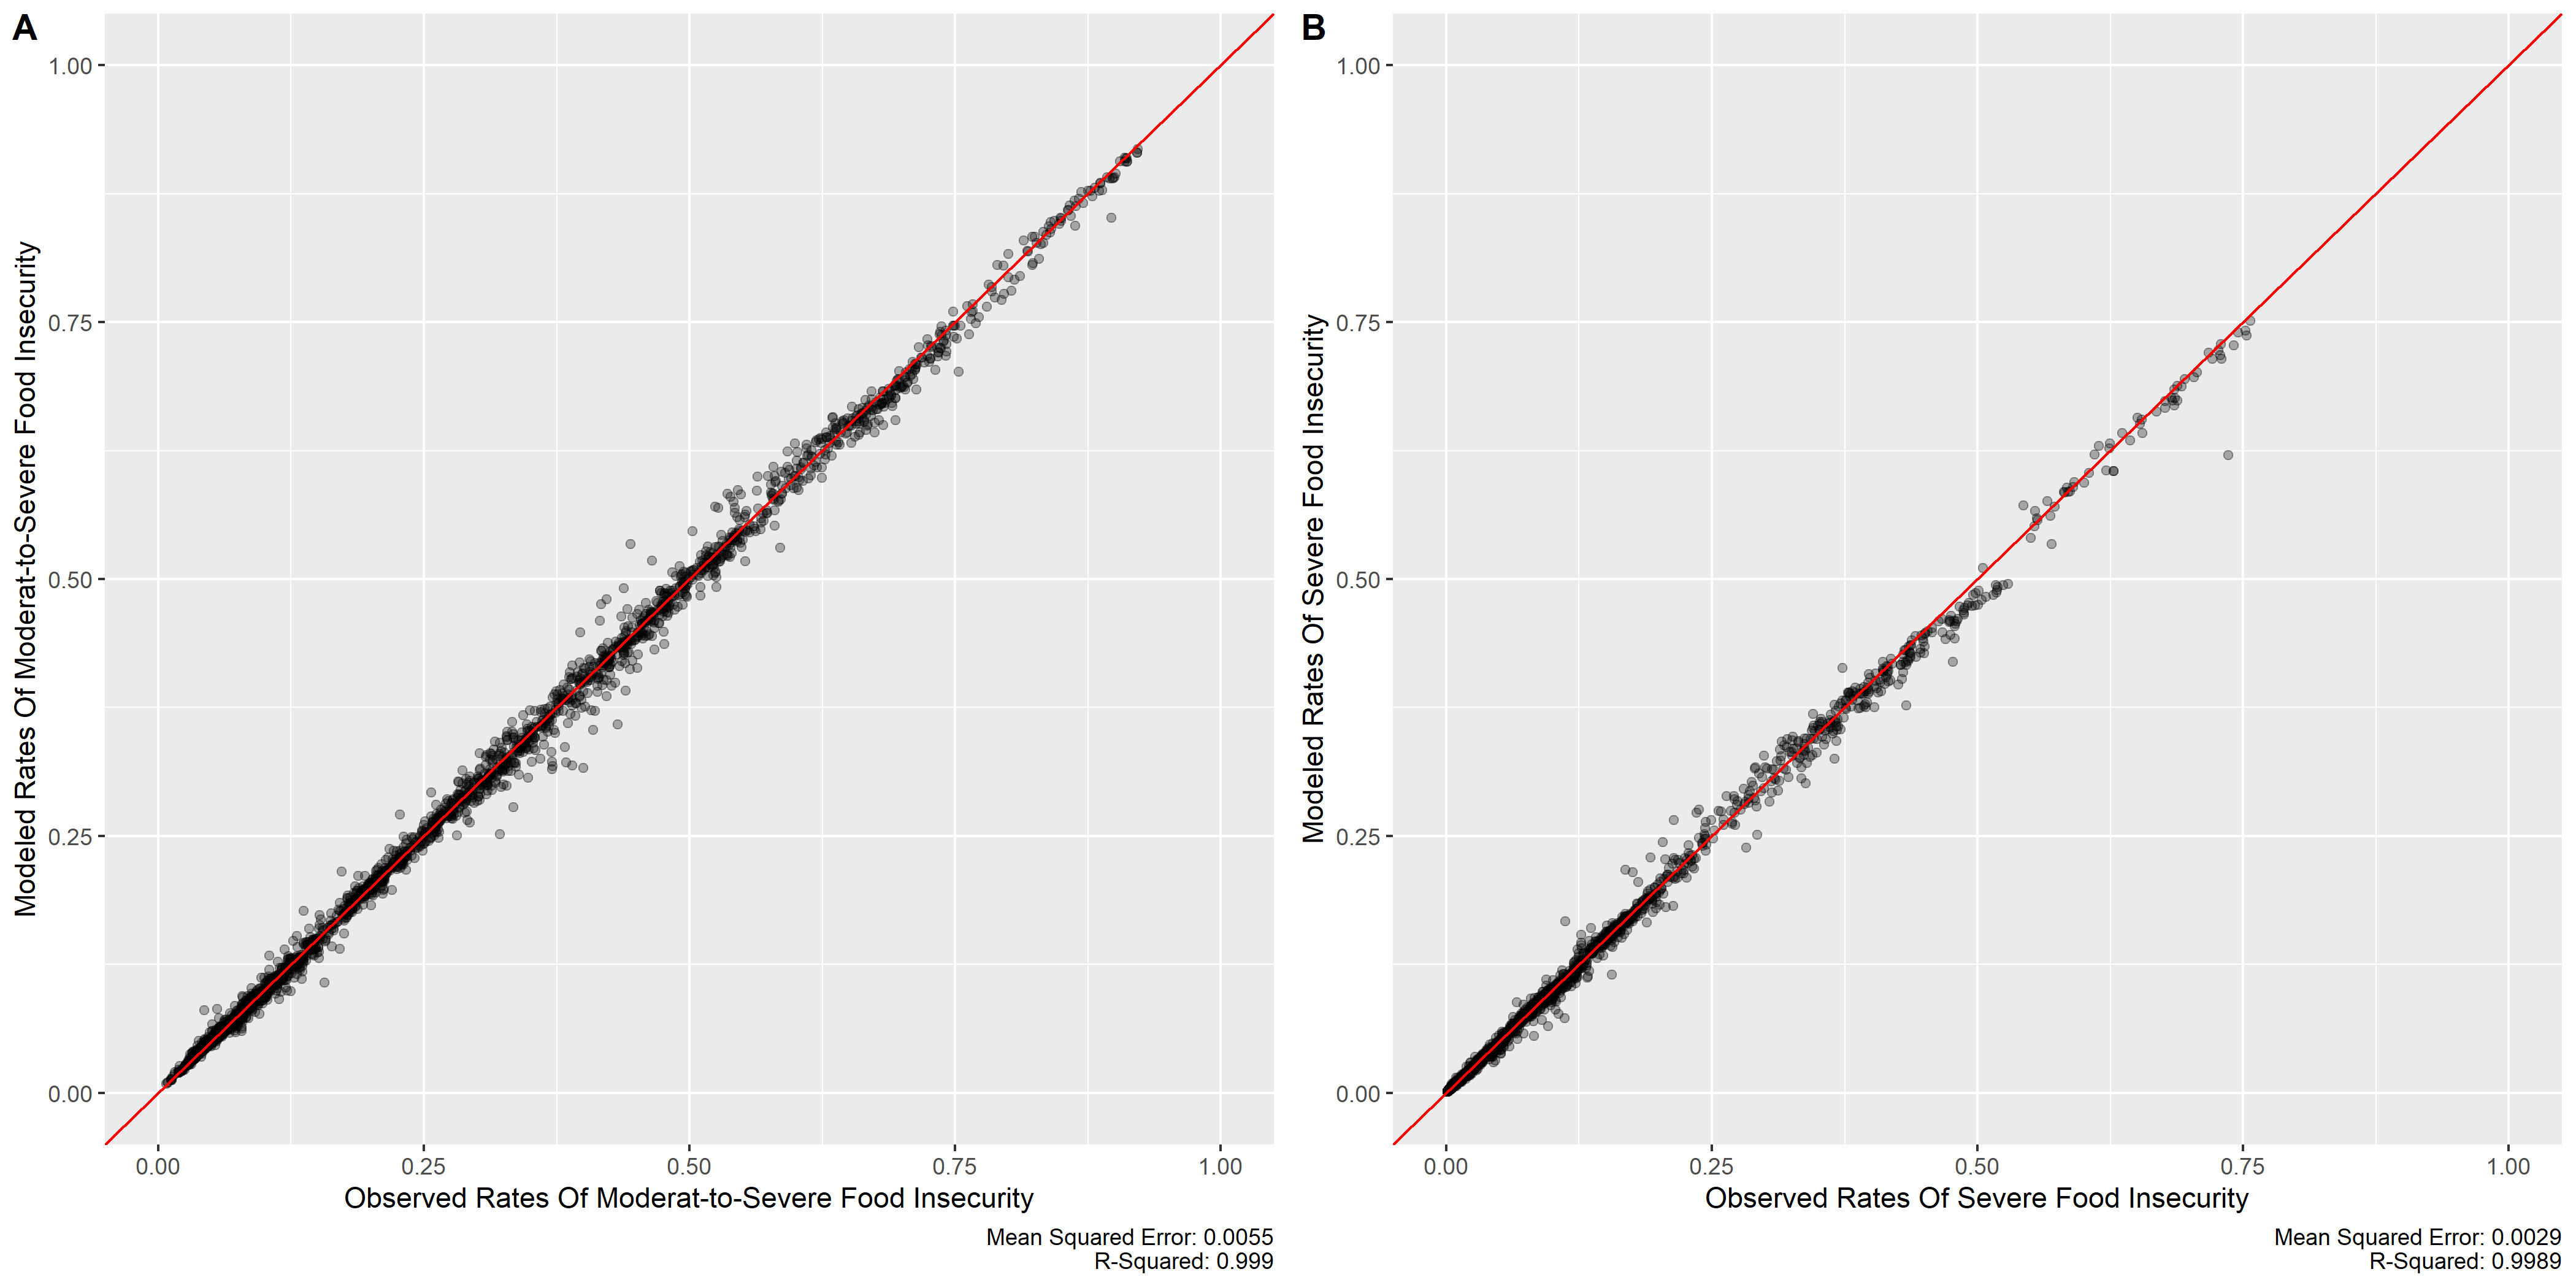
\includegraphics[width=\linewidth]{img/model/in-sample_rf.png}
  \caption{In-Sample Fit of the RF regression model. Panel (A) shows the Moderate-to-Severe model and Panel (B) shows the Severe model.}
  \label{fig:rf_in-sample}
\end{figure}

\begin{figure}[H]
  \centering
  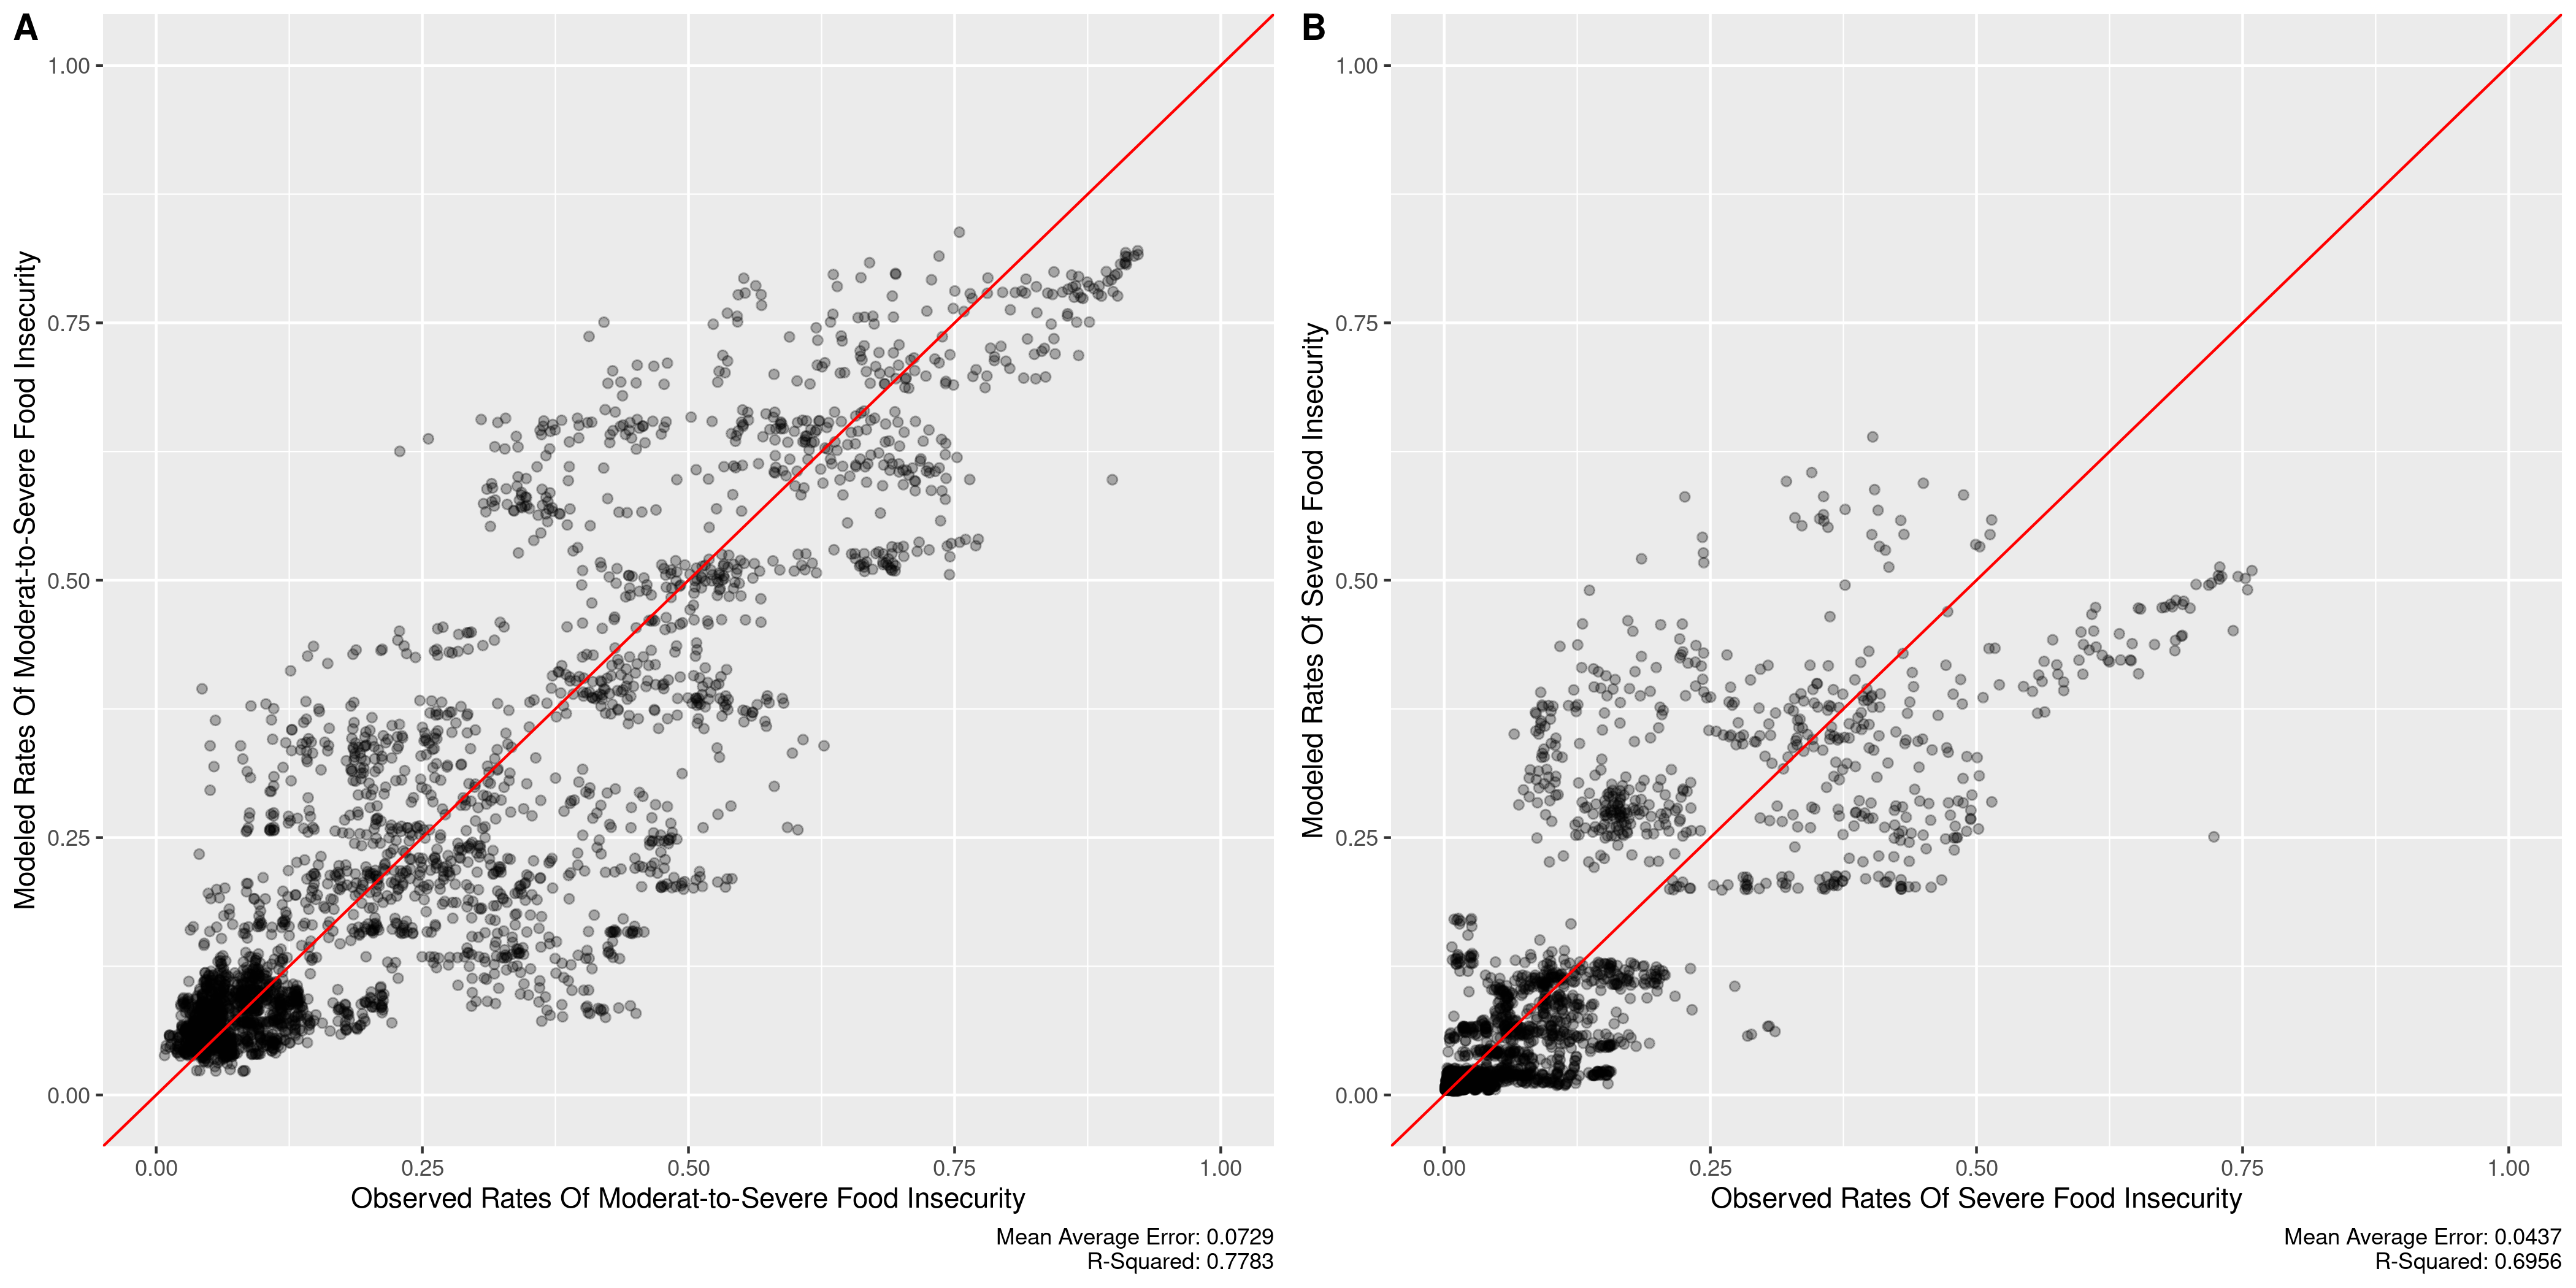
\includegraphics[width=\linewidth]{img/model/out-sample_rf.png}
  \caption{Out-Of-Sample Fit of the RF regression model with 75\% training set and 25\% test set. Panel (A) shows the Moderate-to-Severe model and Panel (B) shows the Severe model.}
  \label{fig:rf_out-sample}
\end{figure}

%HERE EVERYTHING ON THE MODEL, NOT SURE HOW DETAILED
%For modeling the rates of moderate-to-severe and severe food insecurity we use the function \texttt{rfsrc()}. We specify 

\begin{figure}[H]
  \centering
  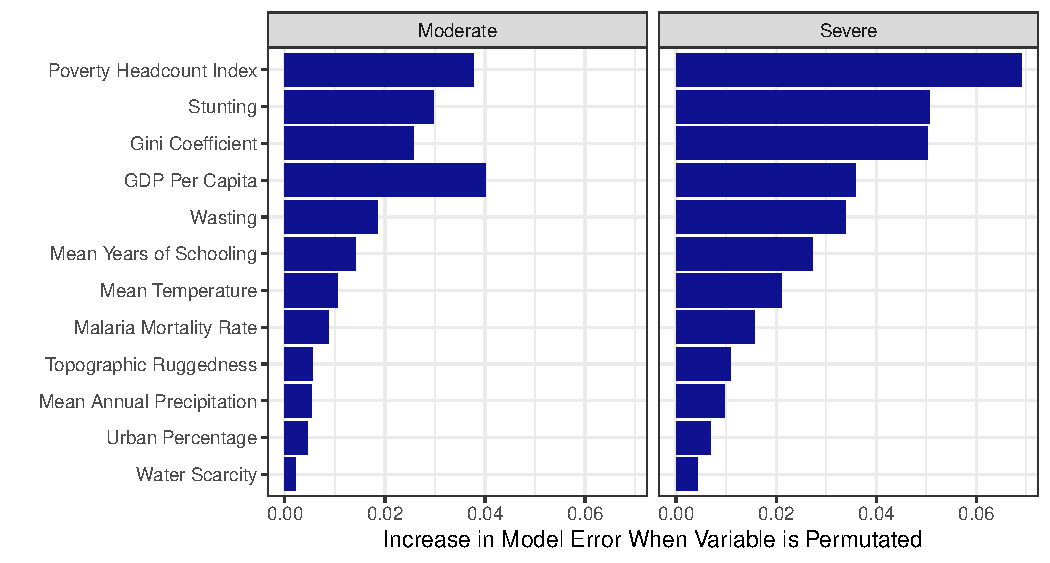
\includegraphics[width=\linewidth]{img/VIMP.pdf}
  \caption{Variable Importance of the RF regression model. Panel (A) shows the Moderate-to-Severe model and Panel (B) shows the Severe model.}
  \label{fig:rf_vimp}
\end{figure}

%https://kogalur.github.io/randomForestSRC/theory.html#section4.2
Lastly we asses the importance of individual variables. This is based on the Breiman-Culter permutation variable importance information \citep{breiman2001random}.  This involved comparing the prediction error on the OOB data to the prediction error of OOB cases where the x-variable $x$ is randomly permutated.  The importance of an individual variable is thus the mean difference between the perturbed and unperturbed error rate, across all trees. 
%MORE INFORMATION HERE
\end{document}
